\documentclass[conference]{IEEEtran}
\IEEEoverridecommandlockouts
% The preceding line is only needed to identify funding in the first footnote. If that is unneeded, please comment it out.
\usepackage{cite}
\usepackage{amsmath,amssymb,amsfonts}
\usepackage{algorithmic}
\usepackage{graphicx}
\usepackage{textcomp}
\usepackage{xcolor}
\usepackage{float}
\usepackage{minted}
\usepackage[colorlinks=true, linkcolor=blue, urlcolor=blue, citecolor=green]{hyperref}
\def\BibTeX{{\rm B\kern-.05em{\sc i\kern-.025em b}\kern-.08em
    T\kern-.1667em\lower.7ex\hbox{E}\kern-.125emX}}
\begin{document}

\title{Parallel Matrix Multiplication\\
}

\author{\IEEEauthorblockN{Luca Falasca}
\IEEEauthorblockA{\textit{0334722} \\
luca.falasca@students.uniroma2.eu
}
\and
\IEEEauthorblockN{Matteo Conti}
\IEEEauthorblockA{\textit{0323728} \\
matteo.conti97@students.uniroma2.eu
}\\
}

\thispagestyle{plain}
\pagestyle{plain}

\maketitle

\begin{abstract}
Il progetto prevede l'implementazione di un nucleo di calcolo per il prodotto tra matrici utilizzando tre approcci distinti: MPI, CUDA e una combinazione di MPI e CUDA. L'approccio MPI sfrutta il paradigma SIMD per la parallelizzazione multiprocesso su CPU, utilizzando tecniche come la block cyclic distribution per la distribuzione del carico tra i processi e la riduzione dei risultati tramite comunicazione collettiva. L'approccio CUDA impiega le potenzialità delle GPU per accelerare le operazioni, con diverse versioni del codice ottimizzate per ridurre il numero di sincronizzazioni e migliorare l'uso della shared memory. La combinazione MPI+CUDA cerca di unire i vantaggi di entrambi i metodi per appianarne gli svantaggi, analizzando un scenario distribuito composto da più macchine con molteplici GPU.
\end{abstract}

\section{Introduzione}
\subsection{Descrizione del problema}
Il progetto verte sulla realizzazione di un nucleo di calcolo per il prodotto tra due matrici, che sia quindi in grado di calcolare
$C \leftarrow C + AB$
dove A è una matrice $M$x$K$ e B è una matrice $K$x$N$. Per le matrici di input, si devono considerare due casi principali:
\begin{enumerate}
    \item Matrici quadrate $M = N = K$;
    \item Matrici rettangolari $M, N \gg K$; con $K = 32, 64, 128, 156$.
\end{enumerate}

\subsection{Obiettivi}
L'obbiettivo di questo progetto è quello di implementare il prodotto tra matrici precedentemente descritto utilizzando tre approcci:
\begin{enumerate}
    \item MPI: utilizzando il paradigma SIMD per la parallelizzazione multiprocesso su CPU
    \item CUDA: sfruttando le potenzialità delle GPU per l'accelerazione delle operazioni computazionali
    \item MPI+CUDA: cercando di combinare i vantaggi delle due tecnologie per appianarne gli svantaggi
\end{enumerate}
\subsection{Metriche di valutazione}
Per valutare le prestazioni delle soluzioni sviluppate sono stati considerati i FLOPS definiti come:
\begin{equation}
    FLOPS = \frac{2MNK}{exec\_time}
\end{equation}
\subsection{Raccolta dei dati}
I dati sono stati raccolti utilizzando il server di dipartimento messo a disposizione per il corso, il quale ha le seguenti specifiche:
\begin{minted}[autogobble, fontsize=\scriptsize, frame=lines]{text}
    Processors: 2 x Intel Xeon Silver 4210
    Memory: 64.0 GiB of RAM
    Video processors: Nvidia Quadro RTX 5000
    CUDA version: 12.3
    MPI version: 4.1
\end{minted}
\section{MPI}
Nel constesto dell'HPC è fondamentale sfruttare le possibilità di parallelizzazione dei task da eseguire, in particolare in questa sezione verrà utilizzato il paradigma SIMD (Single Instruction Multiple Data) per la effettuare la moltiplicazione tra matrici utilizzando le funzionalità offerte da MPI per la parallelizzazione multiprocesso su CPU.\\ In particolare, verranno affrontati i seguenti problemi:
\begin{itemize}
    \item Distribuzione del carico tra i processi
    \item Riduzione del risultato
    \item Implementazione effettiva del prodotto tra matrici
\end{itemize}

\subsection{Distribuzione del carico}
Per la distribuzione del carico è stata adottata una strategia simile a quella adottata dalla libreria ScaLAPACK, cioè la block cyclic distribution. Questa tecnica definisce uno schema per mappare un set di blocchi su dei processi fornendo un bilanciamento del carico ragionevole, è caratterizzata principalmente da due aspetti:
\begin{itemize}
    \item I processi vengono visti come una griglia $P_r$x$P_c$
    \item La matrice viene divisa in blocchi di dimensione $B_r$x$B_c$
\end{itemize}
La griglia dei processi viene fatta scorrere lungo i blocchi con stride pari alla size della griglia, assegnando ad ogni processo $P_{i,j}$ un blocco $B_{i,j}$, ovviamente lo stesso processo in generale riceverà più di un blocco della matrice originale e non per forza tutti i processi riceveranno l'esatto numero di elementi.
Nel nostro caso le matrici sono state distribuite nel seguente modo:
\begin{itemize}
    \item La matrice A è stata distribuita in blocchi quadrati BxB (Fig. \ref{fig:matrix_a_distribution})
    \item La matrice B è stata distribuita in blocchi di righe BxK (Fig. \ref{fig:matrix_b_distribution}), in quanto ogni riga di dimensione B di un blocco della matrice A deve moltiplicare i primi B elementi di ogni colonna della matrice B, questo comporta che i processi nella stessa colonna della process grid debbano ricevere la stessa parte della matrice B
    \item La matrice C è stata distribuita in blocchi righe BxK (Fig. \ref{fig:matrix_c_distribution}), in quanto ogni processo deve calcolare un blocco di dimensione BxK della matrice C, questo comporta che i processi nella stessa riga della process grid debbano ricevere la stessa parte della matrice C
\end{itemize} 
\begin{figure}[H]
    \raggedright
    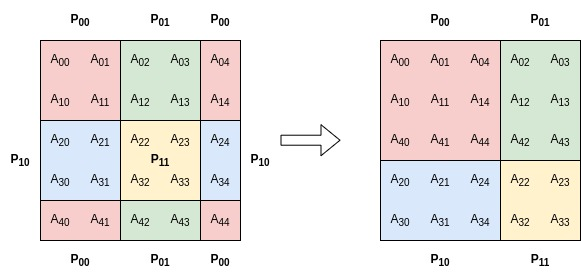
\includegraphics[width=0.45\textwidth]{resources/matrixA_2d_block_cyclic_distribution.jpg}
    \caption{Matrix A distribution.}
    \label{fig:matrix_a_distribution}
\end{figure}
\begin{figure}[H]
    \raggedright
    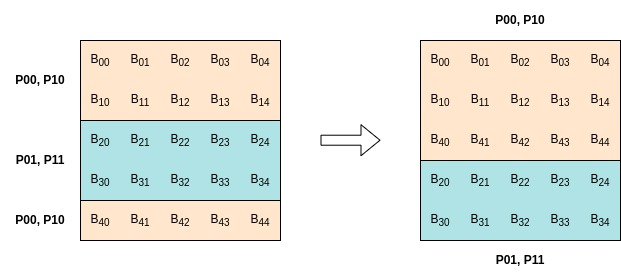
\includegraphics[width=0.45\textwidth]{resources/matrixB_row_block_cyclic_distribution.jpg}
    \caption{Matrix B distribution.}
    \label{fig:matrix_b_distribution}
\end{figure}
\begin{figure}[H]
    \raggedright
    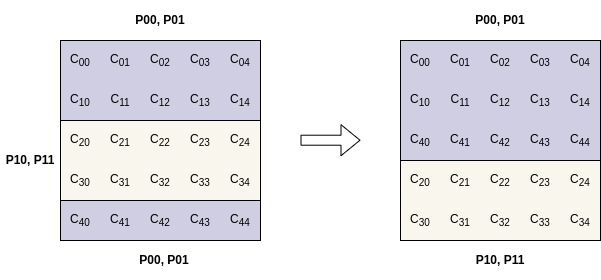
\includegraphics[width=0.45\textwidth]{resources/matrixC_row_block_cyclic_distribution.jpg}
    \caption{Matrix C distribution.}
    \label{fig:matrix_c_distribution}
\end{figure}
Come è possibile notare la differenza tra come è stata distribuita la matrice A e come sono state distribuite le matrici B e C risiede solamente nel come viene vista la process grid e dalla taglia dei blocchi in cui vengono divise le matrici.
Per fare questo è necessario che ogni processo conosca la sua posizione nella process grid, la size della griglia e la size dei blocchi, in modo tale da poter calcolare la porzione di matrice che gli è stata assegnata, in particolare essa viene calcolata da ogni processo come:
\begin{equation}
    \#elem\_block=\#elem\_row\cdot \#elem\_col
\end{equation}
dove $\#elem\_row$ è definito come:
\begin{equation}
    \begin{cases}
        B_c\cdot \#block\_row-(B_c-K \mod B_c) &  \text{if}\ \\
        \text{if}\text{\quad}\text{\quad} P_{i,j} : j=extra\_block\_row-1 \ \land \\ 
        \text{\quad} \text{\quad}K \mod B_c \neq 0\\
        B_c\cdot block\_row & \text{otherwise}\\
    \end{cases} 
\end{equation}
con $\#block\_row$ definito come:
\begin{equation}
    \begin{cases}
        \lfloor\frac{K}{B_c}+1\rfloor &  \text{if}\ P_{i,j} : j<extra\_block\_row \text{\char200{}}\ \text{\char200{}}\ \text{\char200{}}\ \text{\char200{}}\ \text{\char200{}}\ \text{\char200{}}\ \text{\char200{}}\ \text{\char200{}}\ \text{\char200{}}\ \text{\char200{}}\ \text{\char200{}}\ \text{\char200{}}\ \text{\char200{}}\ \text{\char200{}}\ \text{\char200{}}\ \text{\char200{}}\  \\
        \lfloor\frac{K}{B_c}\rfloor & \text{otherwise} \\
    \end{cases} 
\end{equation}
e $\#extra\_block\_row$ definito come:
\begin{equation}
    \begin{cases}
        P_c &  \text{if}\ K \mod B_c \neq 0 \ \land \\
        & \lfloor\frac{K}{B_c}\rfloor \mod B_c=0  \text{\char200{}}\ \text{\char200{}}\ \text{\char200{}}\ \text{\char200{}}\ \text{\char200{}}\ \text{\char200{}}\ \text{\char200{}}\ \text{\char200{}}\ \text{\char200{}}\ \text{\char200{}}\ \text{\char200{}}\ \text{\char200{}}\ \text{\char200{}}\ \text{\char200{}}\ \text{\char200{}}\ \text{\char200{}}\ \text{\char200{}}\ \text{\char200{}}\ \text{\char200{}}\\\
        \lfloor\frac{K}{B_c}\rfloor \mod B_c & \text{otherwise}\\
    \end{cases} 
\end{equation}
In modo analogo è possibile calcolare $\#elem\_col$.
La distribuzione è stata implementata in MPI combinando il tipo \textit{darray} e la funzione \textit{MPI\_File\_open}, in particolare darray permette di definire una vista personalizzata sulla matrice di input, tale il darray verrà utilizzato nell'apertura del file in modo che ogni processo veda solo la sua porzione di matrice, quella che deve ricevere dalla block cyclic distribution. Questo approccio assume che il file contente la matrice risieda su un file system parallelo specifico per HPC, in modo da poterne sfruttare completamente le potenzialità.
\subsection{Riduzione del risultato}
Dopo che ogni processo ha terminato di effettuare la moltiplicazioni tra le sue sottomatrici delle matrici originali, tutti i processi che si trovano sulla stessa riga della process hanno i risultati parziali della stessa parte della matrice C, quindi per ogni riga è necessario effettuare una riduzione che vada a sommare i risultati parziali e ottenere la parte di matrice C finale che appartiene a quella riga, successivamente tale risultato viene scritto su file. E' importante notare che ogni riga di process grid va a lavorare su una parte diversa della matrice C, quindi i processi in una riga della process grid non andranno a scrivere nella stessa zona in cui scrivono i processi di altre righe, tuttavia questo non è vero per i processi all'interno della stessa riga. Per questo motivo si è scelto di introdurre il concetto di \textit{row leader} il quale corrisponde al primo processo di ogni riga della process grid, tale processo in fase di distribuzione del carico sarà l'unico a leggere C ed in fase di riduzione sarà l'unico a scrivere su C, inoltre esso eseguira il prodotto come C=C+A*B mentre gli altri processi nella riga faranno solamente C=A*B. Per la riduzione tramite comunicazione collettiva ogni processo della riga comunichera il suo risultato parziale al row leader il quale effettuerà la somma con il suo risultato parziale, ricevuti tutti i risultati parziali si avrà il risultato completo di una zona di C, la quale verrà scritta su file dal row leader. Questo approccio permette di evitare che i processi nella stessa riga debbano accedere simultaneamente alla stessa zona di file, evitando così problemi di concorrenza e velocizzando la scrittura su file. La riduzione è stata implementata utilizzando la funzione \textit{MPI\_Reduce} con l'operazione di somma utilizzando un comunicatore che definisce la riga della process grid, in cui il root è il row leader.
\begin{figure}[H]
    \centering
    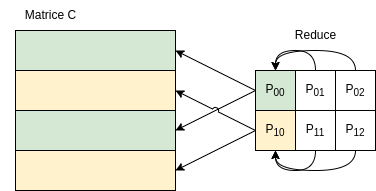
\includegraphics[width=0.5\textwidth]{resources/reduce.png}
    \caption{Reduce con row leader}
    \label{fig:row_leader_reduce}
\end{figure}
\subsection{Implementazione del prodotto}
L'effettiva implementazione del prodotto tra matrici è stata fatta in due modi:
\begin{itemize}
    \item \textit{Naive}, una versione semplice in cui non sono presenti ottimizzazioni per l'accesso in memoria e l'utilizzo della cache
    \item \textit{Column blocked}, una versione più complessa in cui sono presenti ottimizzazioni per l'accesso in memoria e l'utilizzo della cache
\end{itemize}
\subsubsection{Implementazione Naive}
In questa implementazione vengono semplicemente annidati tre cicli for senza tener conto di aspetti come l'accesso in memoria e l'utilizzo della cache.
\subsubsection{Implementazione Column blocked}
In questa implementazione viene tenuto conto dell'ottimizzazione dell'utilizzo della cache e degli accessi in memoria. Quando un elemento di una matrice viene caricato in cache quello che accade è che vengono caricati anche i successivi 15 elementi della stessa riga (utilizzando float con linee di cache da 64byte) è quindi possibile organizzare i cicli for in modo da sfruttare questa caratteristica processando consecutivamente gli elementi che sono stati caricati evitando di doverli ricaricare in futuro.
La soluzione proposta prevede 5 cicli for annidati che si occupano di processare le matrici per blocchi, contribuendo a blocchi di colonne del risultato finale, in particolare:
\begin{itemize}
    \item Il primo ciclo, il più esterno, si occupa di selezionare indici blocchi di colonne della matrice C (Fig. \ref{fig:column_blocked_1})
    \item Il secondo ciclo si occupa scorrere gli indici delle righe dei blocchi di colonne della matrice C selezionate dal precedente ciclo (Fig. \ref{fig:column_blocked_2})
    \item Il terzo ciclo si occupa di scorrere i blocchi di elementi di A e B che contribuiscono al risultato della riga del chunl di colonne di C selezionata nei cicli precedenti (Fig. \ref{fig:column_blocked_3})
    \item Il quarto ciclo si occupa di scorrere gli elementi di A e B nei blocchi selezionati nel ciclo precedente (Fig. \ref{fig:column_blocked_4})
    \item Il quinto ciclo è quello in cui si effettua la moltiplicazione, in particolare fissato un elemento di A esso viene moltiplicato per tutti gli elementi di una riga di B ed inserito nel risultato parziale in C (Fig. \ref{fig:column_blocked_5})
\end{itemize}
\begin{figure}[H]
    \centering
    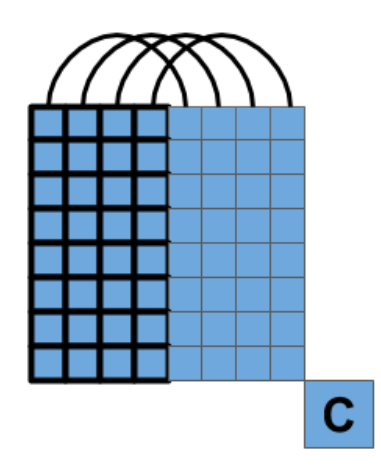
\includegraphics[width=0.2\textwidth]{resources/column_blocked_1.png}
    \caption{Primo ciclo della column blocked multiplication}
    \label{fig:column_blocked_1}
\end{figure}
\begin{figure}[H]
    \centering
    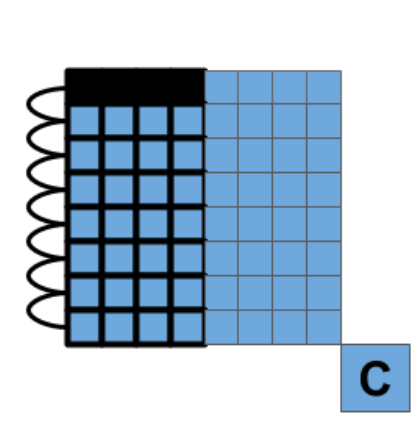
\includegraphics[width=0.2\textwidth]{resources/column_blocked_2.png}
    \caption{Secondo ciclo della column blocked multiplication}
    \label{fig:column_blocked_2}
\end{figure}
\begin{figure}[H]
    \centering
    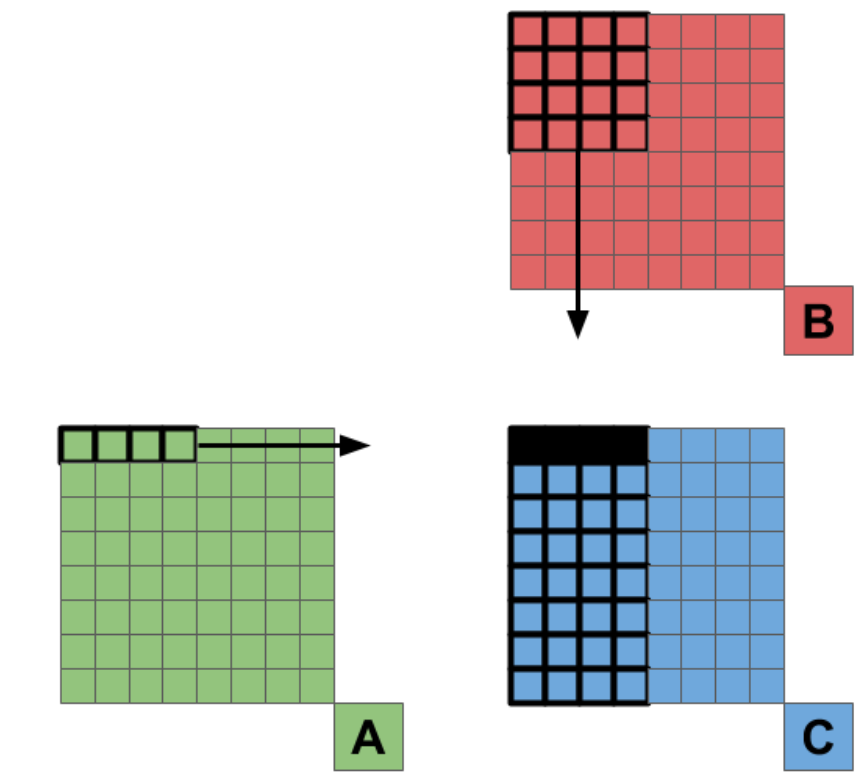
\includegraphics[width=0.35\textwidth]{resources/column_blocked_3.png}
    \caption{Terzo ciclo della column blocked multiplication}
    \label{fig:column_blocked_3}
\end{figure}
\begin{figure}[H]
    \centering
    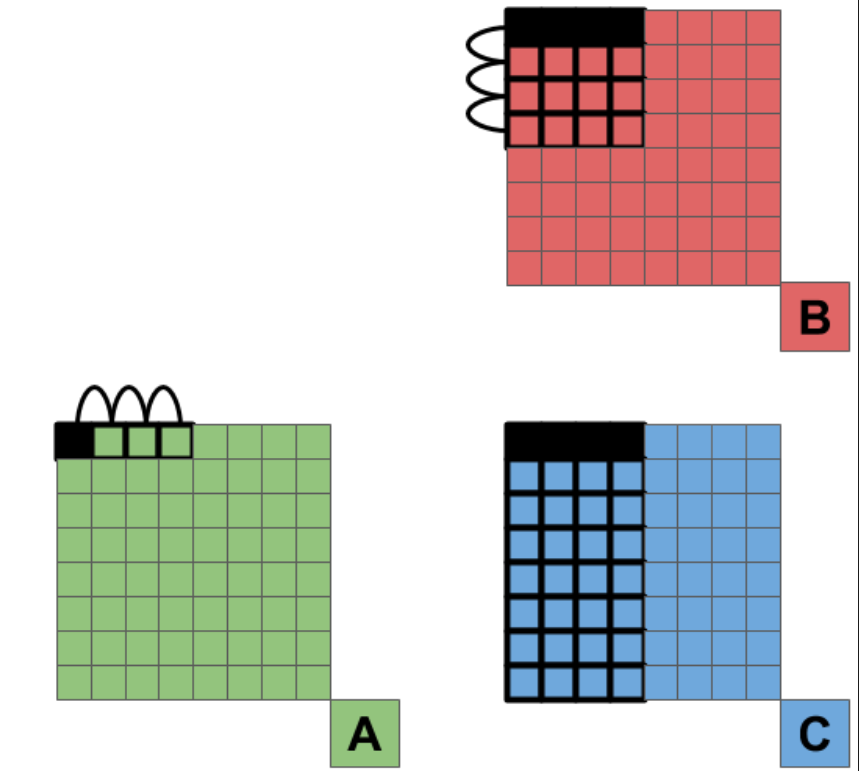
\includegraphics[width=0.35\textwidth]{resources/column_blocked_4.png}
    \caption{Quarto ciclo della column blocked multiplication}
    \label{fig:column_blocked_4}
\end{figure}
\begin{figure}[H]
    \centering
    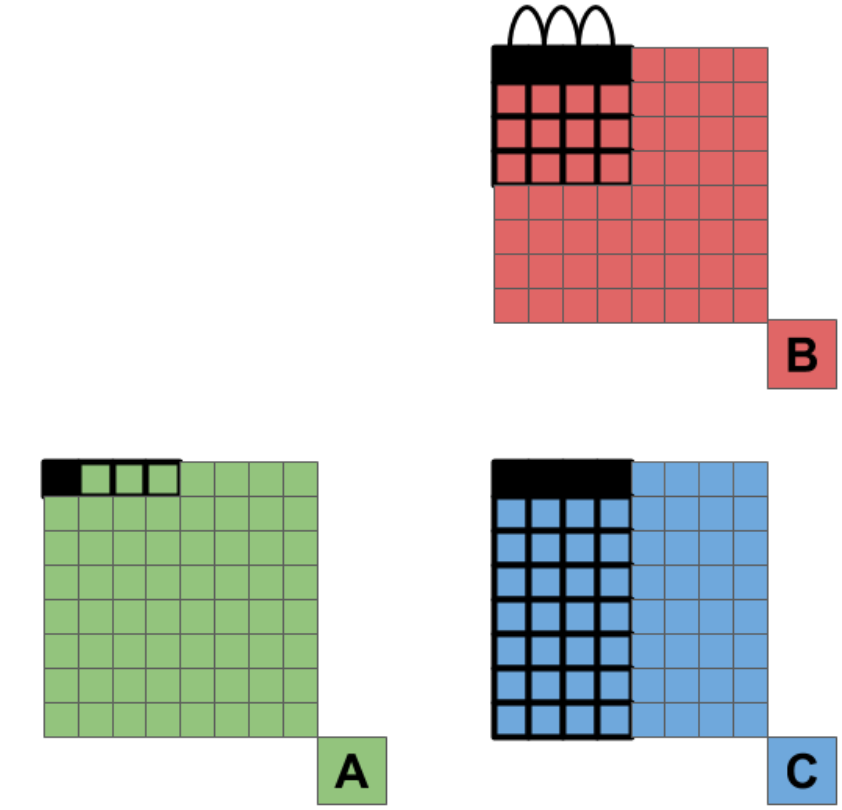
\includegraphics[width=0.35\textwidth]{resources/column_blocked_5.png}
    \caption{Quinto ciclo della column blocked multiplication}
    \label{fig:column_blocked_5}
\end{figure}
\section{CUDA}
Nel contesto dell'elaborazione parallela, l'impiego di unità di elaborazione grafica (GPU) ha rivoluzionato l'accelerazione di operazioni computazionali complesse, tra cui il calcolo matriciale. Questa sezione della relazione si concentra sull'implementazione del calcolo parallelo su GPU per la moltiplicazione di due matrici dense. La moltiplicazione di matrici dense è un'operazione fondamentale in numerose applicazioni scientifiche e di calcolo, tuttavia, il suo impatto computazionale può essere significativo, specialmente con matrici di grandi dimensioni. Pertanto, l'utilizzo delle architetture parallele delle GPU offre un'opportunità significativa per migliorare le prestazioni e ridurre i tempi di calcolo. In questa sezione verranno esaminate diverse implementazioni del prodotto tra matrici su GPU, con l'obiettivo di ottimizzare le prestazioni e ridurre i tempi di esecuzione. All'interno di tutte le versioni del codice la matrice B è stata memorizzata in maniera trasposta perché in questo modo si ottiene un accesso in memoria ottimale, dato che la memorizzazione avviene per righe ed è possibile così sfruttare gli accessi coalizzati alla memoria per i thread nello stesso warp.

\subsection{1 versione}
Nella presente iterazione del codice, si adotta un approccio procedurale mediante il quale la matrice A viene esaminata riga per riga, con ciascuna riga suddivisa per il numero di processi all'interno di un blocco. Analogamente, la matrice B subisce una suddivisione in base al numero di processi. Segue un ciclo in cui ogni processo elabora il proprio elemento della matrice A, effettuando la moltiplicazione con tutti i valori corrispondenti assegnati nella matrice B e sommandoli gradualmente per poi archiviarli in un vettore in memoria condivisa, con indice corrispondente all'identificativo del processo. Ciascun processo esegue tale operazione per tutti gli elementi della riga A che gli sono stati assegnati. Una volta completate le elaborazioni da parte di tutti i processi, si sincronizzano e sommano i risultati parziali ottenuti da ciascun processo mediante l'utilizzo di una funzione di riduzione. Tale procedura viene iterata per tutte le colonne della matrice B. Si è scelto di impiegare blocchi unidimensionali, dove ogni blocco è responsabile di una singola riga della matrice A. Pertanto, il numero di blocchi corrisponde al numero di righe della matrice A (m). (Fig. \ref{fig:cuda_scheme_v1})
\begin{figure}[H]
    \centering
    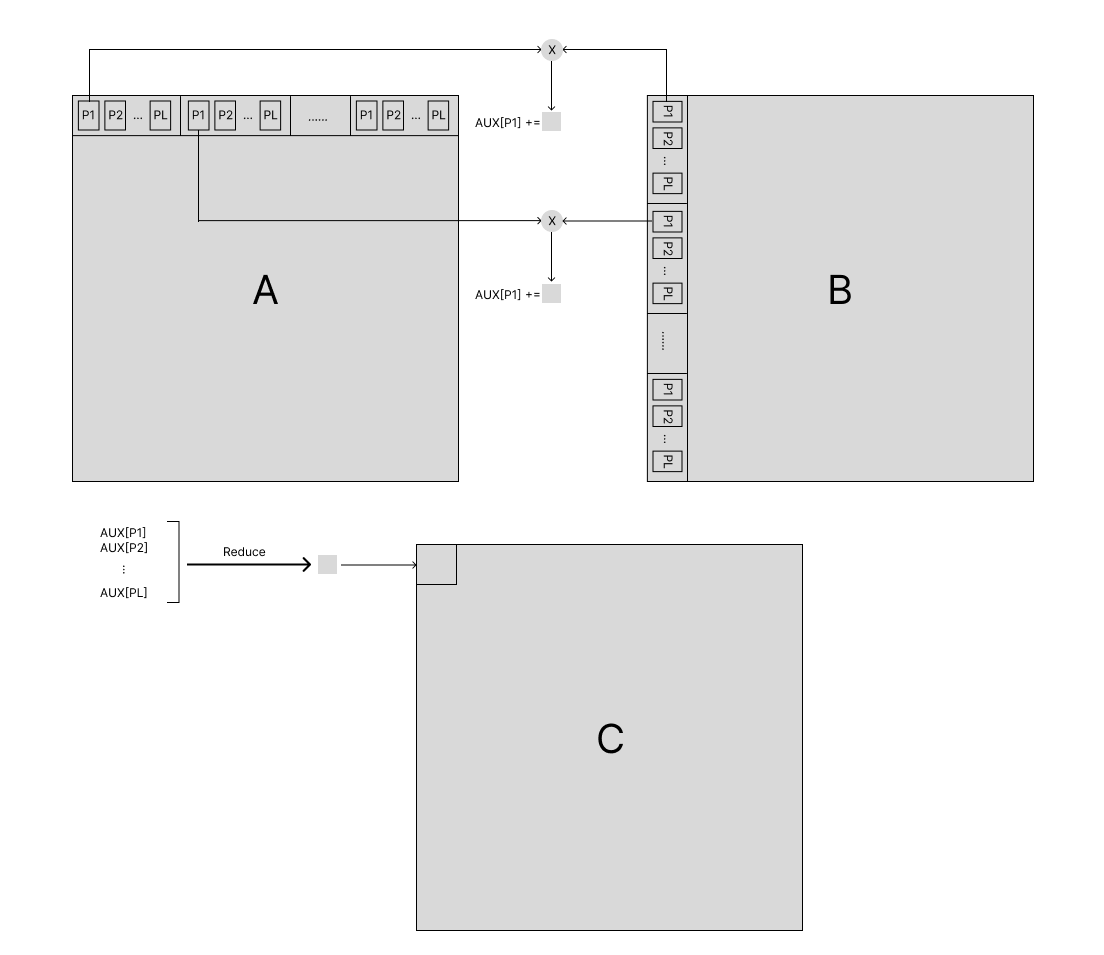
\includegraphics[width=0.5\textwidth]{resources/cuda_scheme_v1.png}
    \caption{Schema di funzionamento della prima versione del codice CUDA.}
    \label{fig:cuda_scheme_v1}
\end{figure}

\subsection{2 versione}
Poiché nella prima versione del codice si scriveva il risultato di un singolo elemento direttamente sulla matrice C ad ogni iterazione sulle colonne, e considerando che tra la fase di calcolo e quella di riduzione si richiedeva una sincronizzazione tra i thread, si è deciso di mitigare l'impatto di tali sincronizzazioni mediante l'adozione di un approccio che prevede l'elaborazione di gruppi di colonne per volta. Di conseguenza, i risultati parziali sono scritti su una matrice temporanea in memoria condivisa. Questa strategia consente di ridurre il numero di sincronizzazioni tra i thread richieste dall'algoritmo. (Fig. \ref{fig:cuda_scheme_v2})


\begin{figure}[H]
    \centering
    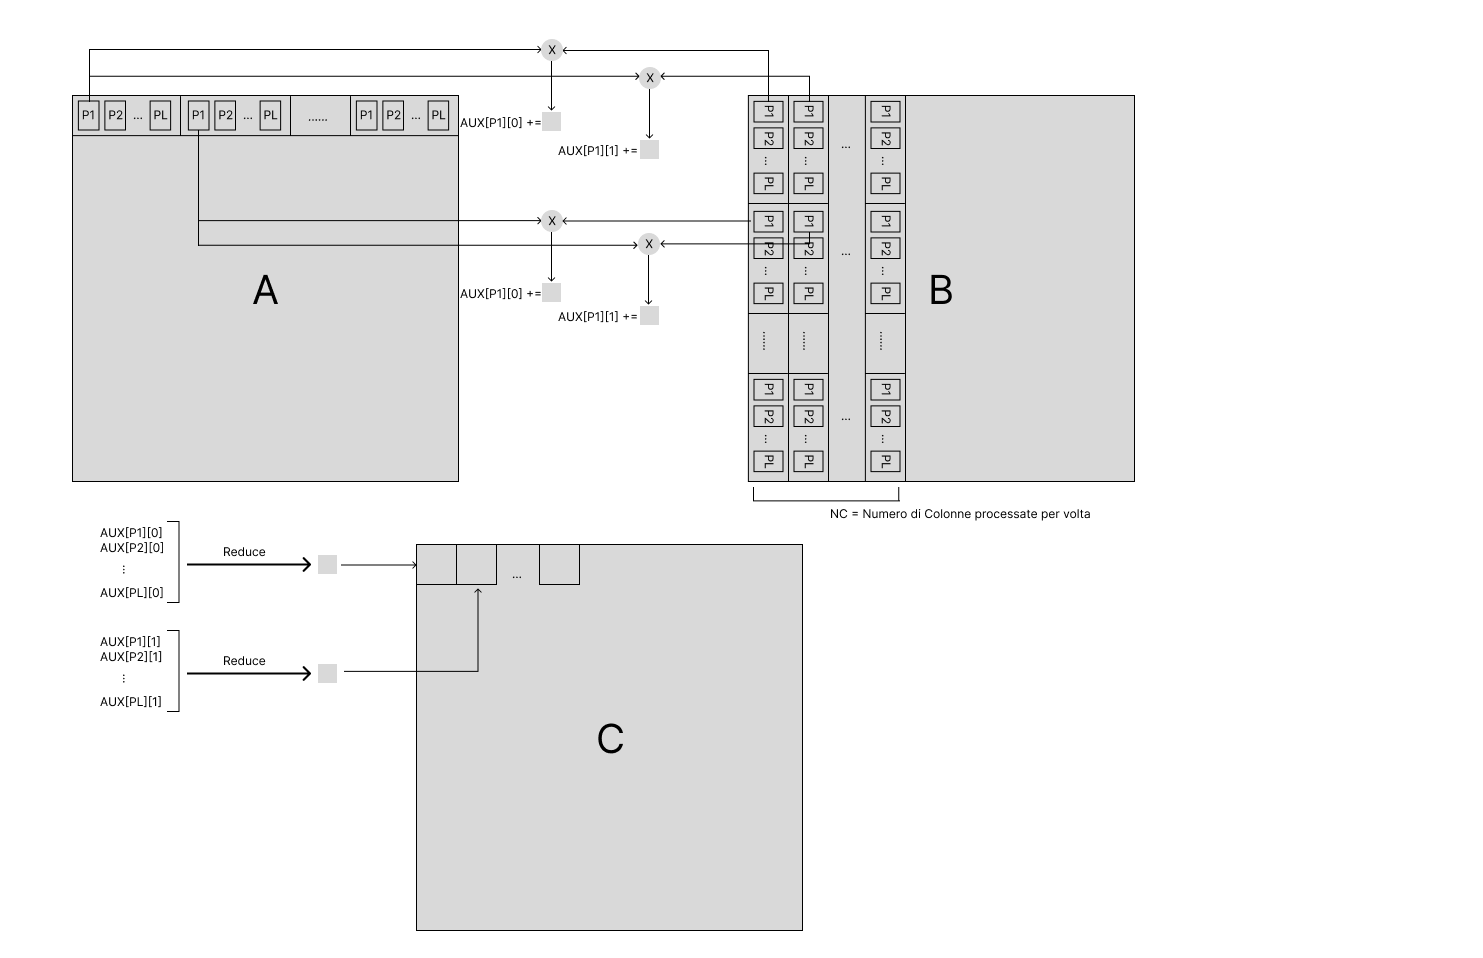
\includegraphics[width=0.5\textwidth]{resources/cuda_scheme_v2.png}
    \caption{Schema di funzionamento della seconda versione del codice CUDA.}
    \label{fig:cuda_scheme_v2}
\end{figure}

\subsection{3 versione}
Nella terza iterazione, si mira a sfruttare l'idea che durante ciascuna iterazione del prodotto tra una riga considerata e un gruppo di colonne, gli stessi elementi della riga A sono utilizzati ripetutamente. Questo consente di memorizzarli in memoria condivisa, riducendo così il numero complessivo di accessi alla memoria globale e incrementando l'efficienza dell'esecuzione. Tuttavia, l'implementazione iniziale prevede lo scorrimento di una colonna alla volta, il che implica la necessità di memorizzare l'intera riga in memoria condivisa. Questo approccio risulta poco pratico dato che le dimensioni delle righe sono considerevoli e la capacità della memoria condivisa è limitata. \\ Per risolvere questo problema, anziché iterare una colonna per volta, si è optato per l'iterazione sulla riga parziale del sottoinsieme delle colonne di B per volta. In questo modo, viene sfruttata la medesima porzione della riga A per eseguire il prodotto con le colonne di B. Tale strategia ottimizza l'utilizzo della memoria condivisa, garantendo al contempo un migliore bilanciamento tra l'efficienza computazionale e l'utilizzo delle risorse di memoria disponibili. (Fig. \ref{fig:cuda_scheme_v3})

\begin{figure}[H]
    \centering
    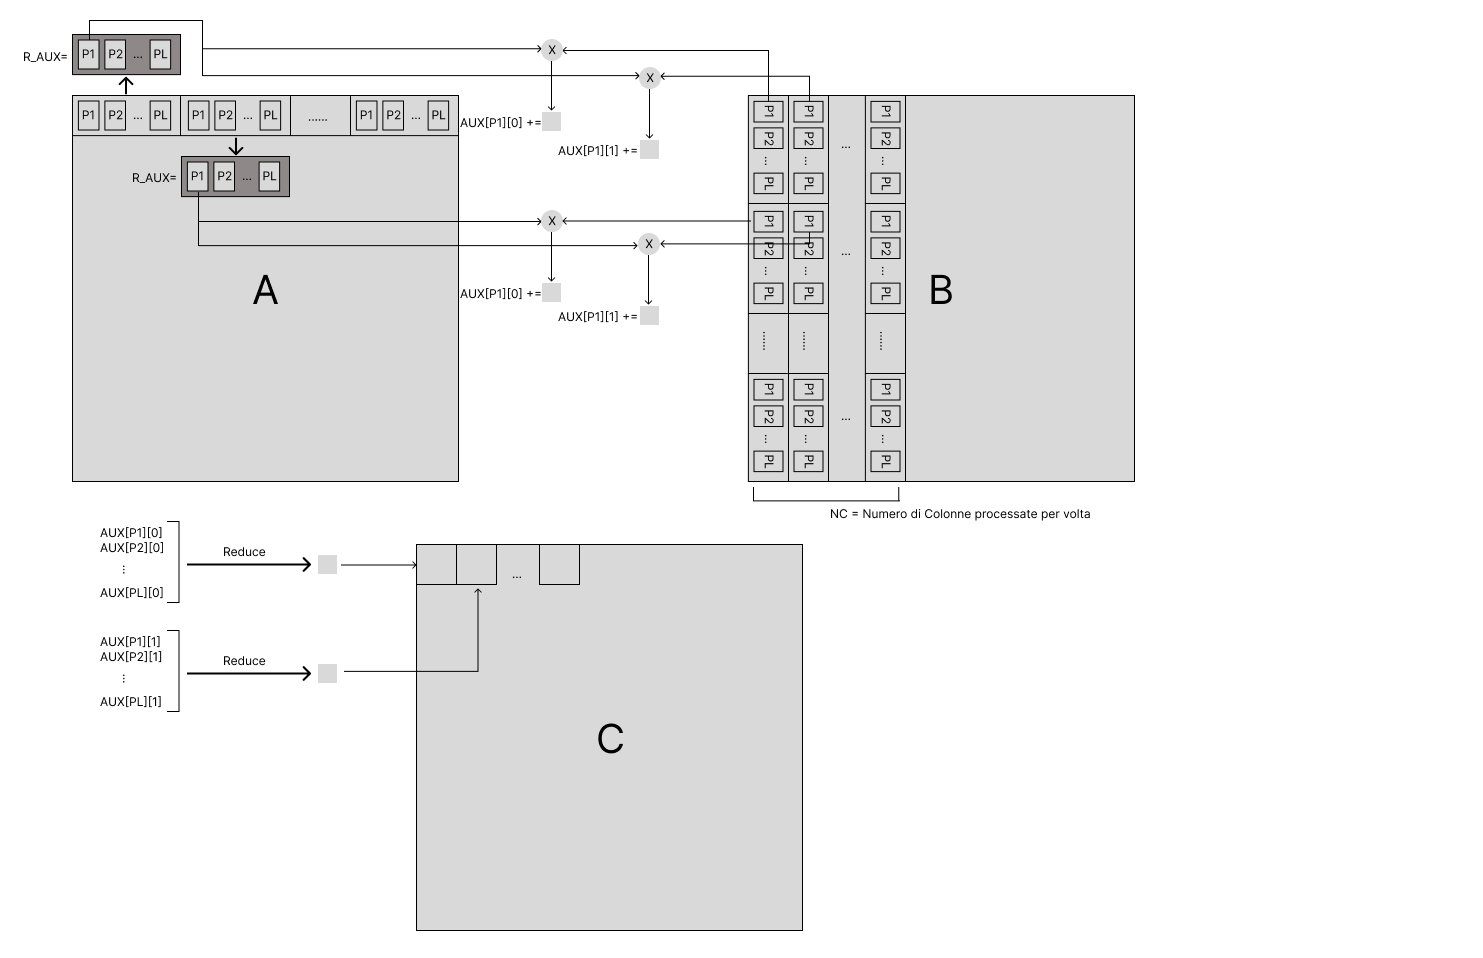
\includegraphics[width=0.5\textwidth]{resources/cuda_scheme_v3.png}
    \caption{Schema di funzionamento della terza versione del codice CUDA.}
    \label{fig:cuda_scheme_v3}
\end{figure}

\subsection{Configurazione dei parametri}
\subsubsection{Thread}
Nelle varie implementazioni è stata utilizzata una griglia unidimensionale di dimensione pari al numero di righe della matrice A. Questo è dovuto al fatto che ogni blocco è responsabile di una singola riga della matrice A. 
Per quanto riguarda il numero di thread per ogni blocco (block size), si è scelto di utilizzare un valore pari a 256, in quanto si è rivelato il più efficiente in termini di prestazioni. In generale a parte mantenere il numero di thread multiplo di 32 è difficile stabilire un valore ottimale, in quanto dipende da molti fattori, per questo motivo si è scelto di utilizzare un valore che si è rivelato efficiente in base ai test effettuati.
\subsubsection{Shared memory}
La shared memory nella prima versione è stata utilizzata per memorizzare i risultati parziali ottenuti da ciascun thread e la dimensione dell'array è stata impostata in base al numero di thread per blocco. Nella seconda versione si usa invece una matrice in shared memory che dipende dal numero di colonne scelte. Quindi ha senso scegliere un numero di colonne che massimizzi la shared memory disponibile. Tuttavia facendo diverse prove in fase di sviluppo è stato notato che massimizzare l'utilizzo della shared memory non porta alle migliori prestazioni e quindi è stata scelta la combinazione tra numero di processi e numero di colonne che si è rivelata più efficiente. Nel nostro caso la seguente combinazione è quella con 256 thread e 28 colonne per volta. Quindi tutti gli esperimenti successivi sono stati fatti con questa configurazione.
\subsubsection{Bank conflict}
Andiamo ad analizzare il problema dei bank conflict nel nostro contesto. Verrà analizzata solo la versione 3 perché tutti gli altri casi sono sottoinsiemi di questo.\\
Nella versione 3 del codice per GPU ci sono 2 possibili utilizzi della shared memory: 
\begin{itemize}
    \item Memorizzare la riga della matrice A 
    \item Memorizzare un dato numero di colonne della matrice B
\end{itemize}
Per quanto riguarda il primo caso, la quantità di shared memory utilizzata è pari al numero di thread in un blocco, il quale è multilpo di 32. Il che significa che ogni warp di thread utilizza 32 banchi per volta e accedendo in questo modo in maniera simultanea alla memoria. Nell'utilizzo che se ne fa nell'algoritmo ogni thread accede ad una bank diverso, quindi non ci possono essere conflitti perché il pattern di accesso è lineare con stride di una word da 32 bit, dato che vengono utilizzati i float che occupano 4 byte.\\
Per quanto riguarda il secondo caso, la shared memory viene utilizzata per mantenere i risultati parziali. Ma anche in questo caso il pattern di accesso è identico al primo caso, perché ad ogni thread è associato un vettore di risultati parziali ed ognuno accede ad un banco diverso dato che il vettore bidimensionale in shared memory segue un row-major order. il vettore ausiliario è fatto nel seguente modo:
\[
aux = \left[
\begin{matrix}
pr_{col_0, t_0} & pr_{col_0, t_2} & ... & pr_{col_0, t_{BD}} \\
pr_{col_1, t_0} & pr_{col_1, t_2} & ... & pr_{col_1, t_{BD}} \\
... & ... & ... & ... \\
pr_{col_{Q}, t_0} & pr_{col_{Q}, t_2} & ... & pr_{col_{Q}, t_{BD}}
\end{matrix}\right]
\]
dove $Q$ è il numero di colonne scelte per iterazione e $BD$ è la dimensione del blocco di thread, che corrisponde quindi al numero di thread impiegati.\\
Ogni thread accede quindi ad un'area contigua rispetto agli altri thread, e dato che essi sono in multiplo di 32 andranno ad eseguire accessi coalizzati alla shared memory all'interno dei warp.

%MPI + CUDA
\section{MPI+CUDA}
Questo approccio cerca di combinare i vantaggi dati dalla soluzione MPI e dalla soluzione CUDA. L'utilizzo della soluzione CUDA ci permette di ottenere un miglioramento delle performance molto grande rispetto all utilizzo della sola CPU però ha il limite di essere vincolato alla memoria ed al numero di GPU del singolo server, con l'utilizzo della soluzione MPI si cerca di risolvere proprio questo problema sfruttanto la possibilità di poter utilizzare le GPU dell'intero cluster e sfruttare l'astrazione di memoria distribuita. Per come è fatta la soluzione MPI è possibile effettuare la block cyclic distribution su un intero cluster di server senza che ogni server debba leggere l'intero problema, questo ci permette di risolvere il problema della dimensione della memoria dei singoli server che ora leggeranno solo la loro sottomatrice. Inoltre in questo modo non si è vincolati al numero di GPU di un singolo server, ma è possibile utilizzare le GPU dell'intero cluster, ogni server andrà ad eseguire la computazione accelerata sulla sottomatrice che gli è stata assegnata tramite block cyclic distribution e successivamente verrà effettuata la riduzione dei risultati parziali sui server che accolongono i \textit{row leader} che si occuperanno di scrivere il risultato finale su file. In questo caso è possibile notare come l'utilizzo dei row leader favorisca la scalabilità in fase di riduzione in quanto non si ha un unico server che deve ridurre i risultati di tutto il cluster.
\begin{figure}[H]
    \centering
    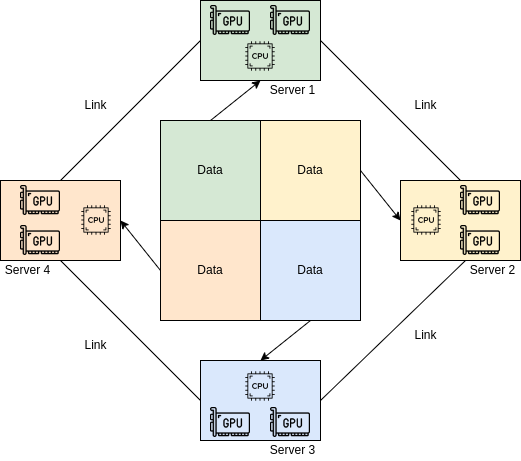
\includegraphics[width=0.4\textwidth]{resources/mpi_cuda_adjusted.png}
    \caption{Schema di funzionamento della soluzione MPI+CUDA.}
    \label{fig:mpi_cuda_scheme}
\end{figure}

\section{Analisi delle prestazioni}
\subsection{MPI}
Di seguito vengono riportati i risultati ottenuti nell'implementazione MPI al variare di:
\begin{itemize}
    \item Numero di processi
    \item Dimensione delle matrici
    \item Implementazione del prodotto
\end{itemize}
Per tutti i calcoli sono stati utilizzati blocchi $32x32$ ed i processi sono stati organizzati in una griglia quadrata ove possibile (16 processi griglia $4x4$, 20 processi griglia $5x4$)

%RISULTATI MPI QUADRATE
\subsubsection{Matrici quadrate}
Come è possibile vedere dai grafici in Fig. \ref{fig:square_matrix_naive} e \ref{fig:square_matrix_blocked}, all'aumentare del numero di processi si hanno sempre vantaggi abbastanza consistenti che diventano più evidenti all'aumentare della dimensione del problema fino ad arrivare ad un fattore 30, inoltre si può vedere come l'implementazione column blocked del prodotto porti un miglioramento molto consistente delle prestazioni arrivando ad un fattore 2. Dai grafici è inoltre possibile vedere dei drastici cali di performance, essi avvengono in corrispondenza di matrici le cui dimensioni sono potenze di 2 e peggiorano con l'aumentare della taglia del problema. Questo degrado delle performance è probabilmente un fatto dovuto a problemi di cache, in particolare al problema del \textit{critical stride}\cite{b1}, nella trattazione viene spiegato come avere zone di memoria la cui taglia che è multiplo del critical stride porti a problemi di cache che si manifestano come un calo di performance molto consistente. Il critical stride puo essere calcolato come:
\begin{equation}
    critical\_stride = cache\_line\_size \cdot associativity
\end{equation}
Nel nostro caso le linee di cache hanno taglia 64B mentre l'associatività e 8-way pertanto il critical stride risulta essere 512B, il che è plausibile in quanto il degrado delle performance è osservabile dalle matrici $512x512$ in poi, in particolare per 1024, 2048, 4096, 8192 dove ad esempio nel caso di matrici $4096x4096$ con blocchi $32x32$ e 4 processi organizzati in una griglia $2x2$ si ha che ogni processo riceve dalla block cyclic distribuzion una matrice $2048x2048$ le cui dimensioni sono ancora multiplo del critical stride, questo rimane vero anche con più processi ad esempio 16 processi in griglia $4x4$ si avrebbe che ogni processo riceve una matrice $1024x1024$.
Per questioni di tempo non sono state implementate le soluzioni proposte in \cite{b1} per risolvere il problema. Un'altra possibile soluzione al problema è quella di cambiare la taglia dei blocchi utilizzati nella block cyclic distribution, in modo tale da evitare che le dimensioni delle matrici distribuite siano multiplo del critical stride, per questioni di tempo e occupazione del server non sono stati effettuati test in tal senso.

In Fig. \ref{fig:square_matrix_naive_nocrit} e \ref{fig:square_matrix_blocked_nocrit} sono riportati i risultati ottenuti senza il problema del critical stride per poter visualizzare meglio l'andamento delle performance.
\begin{figure}[H]
    \centering
    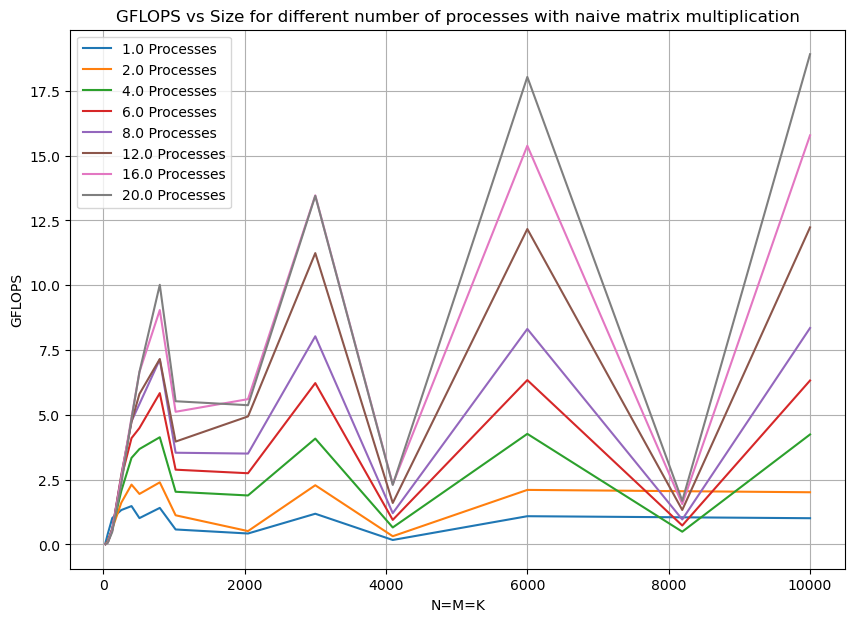
\includegraphics[width=0.4\textwidth]{resources/quadrate_naive.png}
    \caption{Prestazioni ottenute con matrici quadrate e prodotto naive.}
    \label{fig:square_matrix_naive}
\end{figure}
\begin{figure}[H]
    \centering
    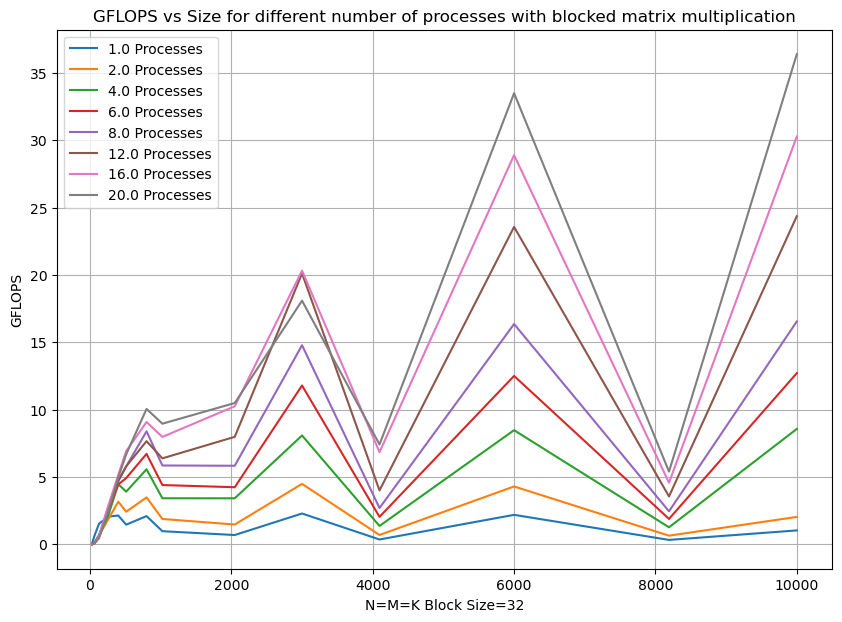
\includegraphics[width=0.4\textwidth]{resources/quadrate_blocked.png}
    \caption{Prestazioni ottenute con matrici quadrate e prodotto column blocked.}
    \label{fig:square_matrix_blocked}
\end{figure}
\begin{figure}[H]
    \centering
    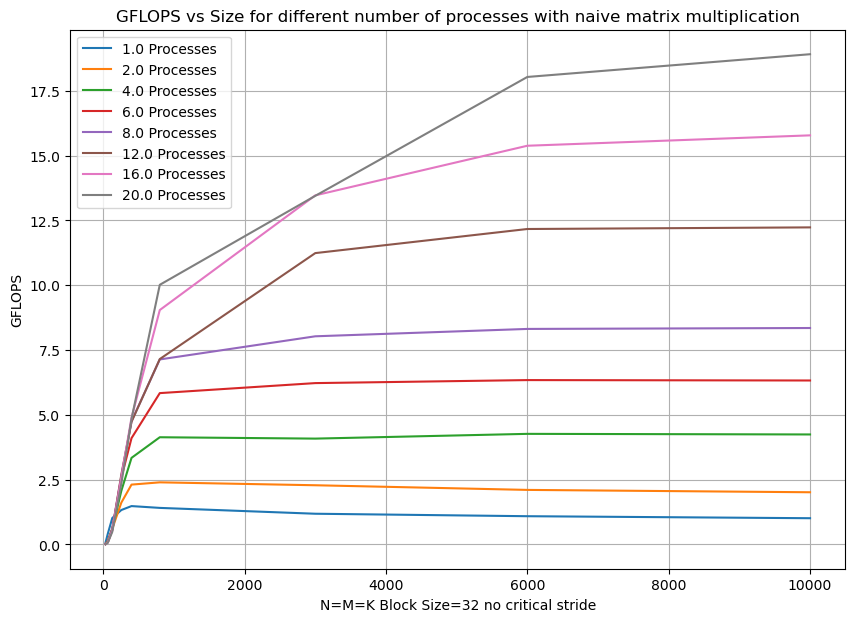
\includegraphics[width=0.4\textwidth]{resources/square_naive_nocrit.png}
    \caption{Prestazioni ottenute con matrici quadrate e prodotto naive senza critical stride.}
    \label{fig:square_matrix_naive_nocrit}
\end{figure}
\begin{figure}[H]
    \centering
    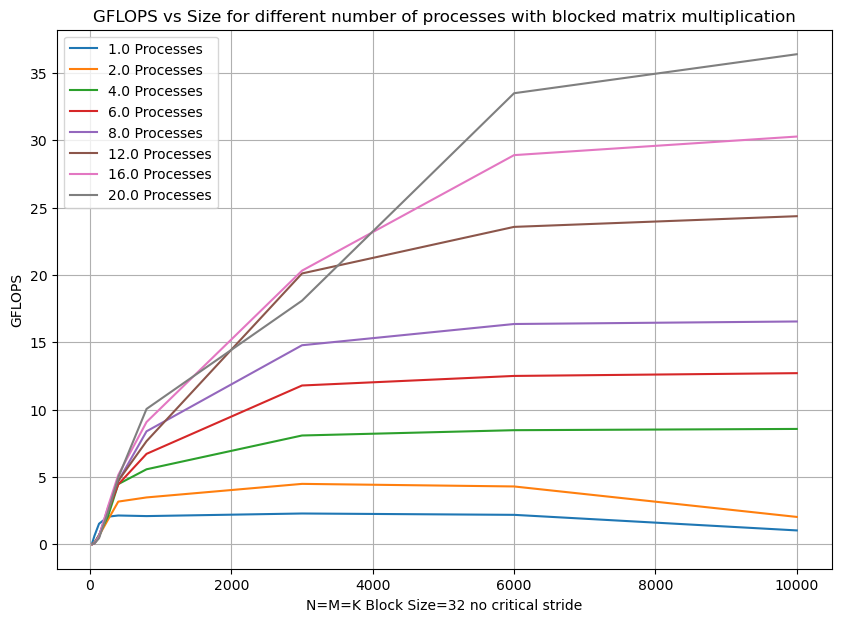
\includegraphics[width=0.4\textwidth]{resources/square_blocked_nocrit.png}
    \caption{Prestazioni ottenute con matrici quadrate e prodotto column blocked senza critical stride.}
    \label{fig:square_matrix_blocked_nocrit}
\end{figure}
%RISULTATI MPI RETTANGOLARI
\subsubsection{Matrici rettangolari}
Come è possibile vedere dai grafici in Fig. \ref{fig:rect_k32_matrix_naive}, \ref{fig:rect_k32_matrix_blocked}, \ref{fig:rect_k64_matrix_naive}, \ref{fig:rect_k64_matrix_blocked}, \ref{fig:rect_k128_matrix_naive}, \ref{fig:rect_k128_matrix_blocked}, \ref{fig:rect_k156_matrix_naive} e \ref{fig:rect_k156_matrix_blocked} anche in questo caso la parallelizzazione porta ad un vantaggio abbastanza evidente, tuttavia non sempre il numero massimo di processi disponibili porta ai risultati migliori, ad esempio nel caso di $K=32$ e $K=64$ effettuare il calcolo con 2, 8 e 12 processi porta a prestazioni migliori rispetto al calcolo con 20 processi, per $K=128$ risulta essere migliore il calcolo effettuato con 16 processi mentre con $K=156$ risultano migliori 12 e 16 processi. Questo comportamento è probabilmente dovuto al fatto che rispetto alle matrici quadrate la taglia del problema è molto più piccola, infatti in tutti i casi l'utilizzare un minor numero di processi porta a vantaggi di solo 1 o 2 GFlops che sono trascurabili rispetto ai vantaggi ottenuti con le matrici quadrate. Inoltre si può notare come l'implementazione column blocked porti sempre a prestazioni migliori rispetto a quella naive, anche se in modo meno evidente rispetto alle matrici quadrate, questo probabilmente è sempre dovuto alla taglia del problema.
Come è possibile vedere dai grafici anche in questo caso, seppur in maniera meno evidente, è presente il problema del \textit{critical stride}, in Fig. \ref{fig:rect_k32_matrix_naive_nocrit}, \ref{fig:rect_k32_matrix_blocked_nocrit}, \ref{fig:rect_k64_matrix_naive_nocrit}, \ref{fig:rect_k64_matrix_blocked_nocrit}, \ref{fig:rect_k128_matrix_naive_nocrit}, \ref{fig:rect_k128_matrix_blocked_nocrit}, \ref{fig:rect_k156_matrix_naive_nocrit} e \ref{fig:rect_k156_matrix_blocked_nocrit} sono riportati i risultati ottenuti senza il problema del critical stride per poter visualizzare meglio l'andamento delle performance.
\begin{figure}[H]
    \centering
    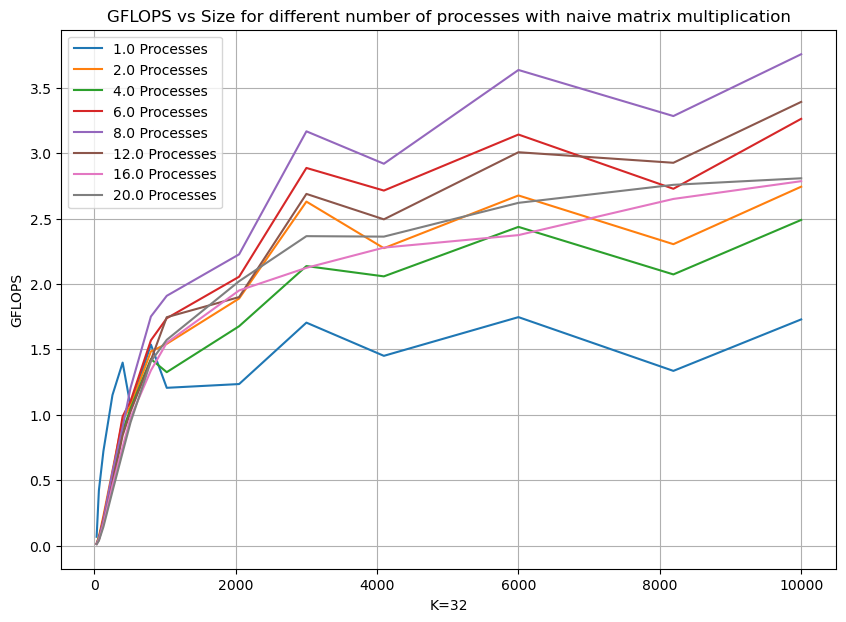
\includegraphics[width=0.4\textwidth]{resources/rettangolari_k32_naive.png}
    \caption{Prestazioni ottenute con matrici rettangolari K=32 e prodotto naive.}
    \label{fig:rect_k32_matrix_naive}
\end{figure}
\begin{figure}[H]
    \centering
    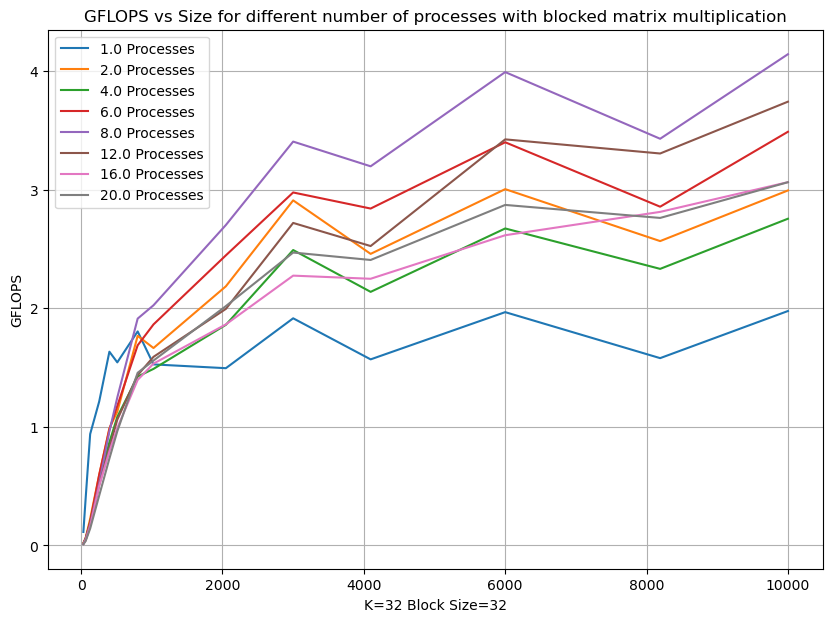
\includegraphics[width=0.4\textwidth]{resources/rettangolari_k32_blocked.png}
    \caption{Prestazioni ottenute con matrici rettangolari K=32 e prodotto column blocked.}
    \label{fig:rect_k32_matrix_blocked}
\end{figure}
\begin{figure}[H]
    \centering
    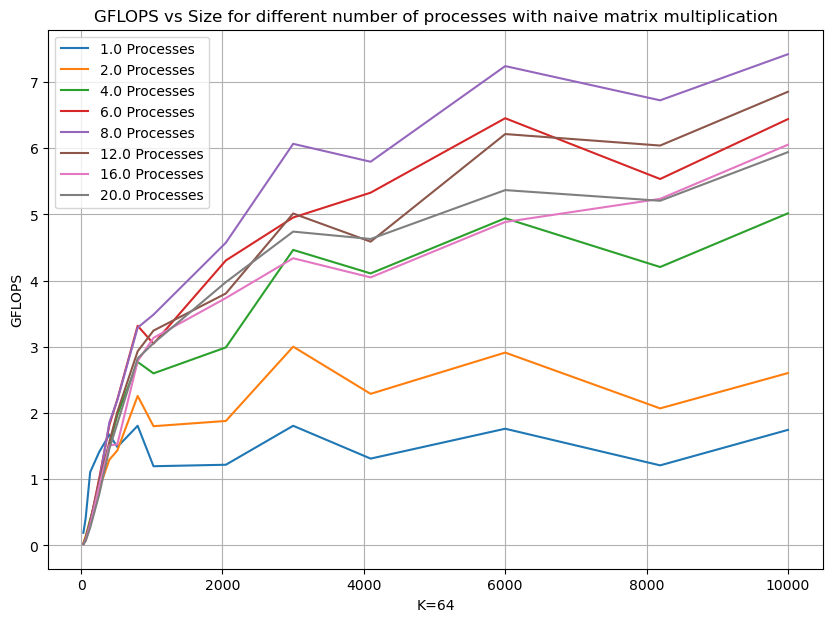
\includegraphics[width=0.4\textwidth]{resources/rettangolari_k64_naive.png}
    \caption{Prestazioni ottenute con matrici rettangolari K=64 e prodotto naive.}
    \label{fig:rect_k64_matrix_naive}
\end{figure}
\begin{figure}[H]
    \centering
    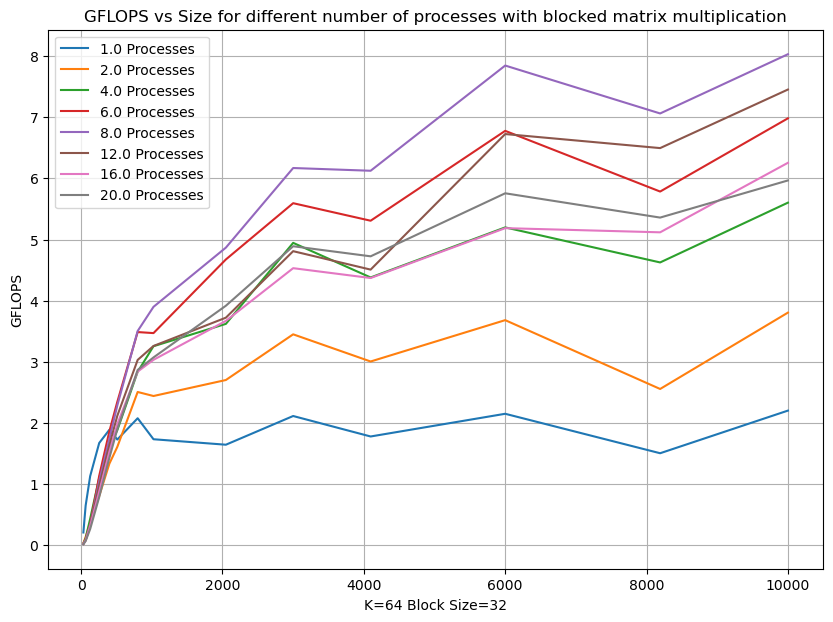
\includegraphics[width=0.4\textwidth]{resources/rettangolari_k64_blocked.png}
    \caption{Prestazioni ottenute con matrici rettangolari K=64 e prodotto column blocked.}
    \label{fig:rect_k64_matrix_blocked}
\end{figure}
\begin{figure}[H]
    \centering
    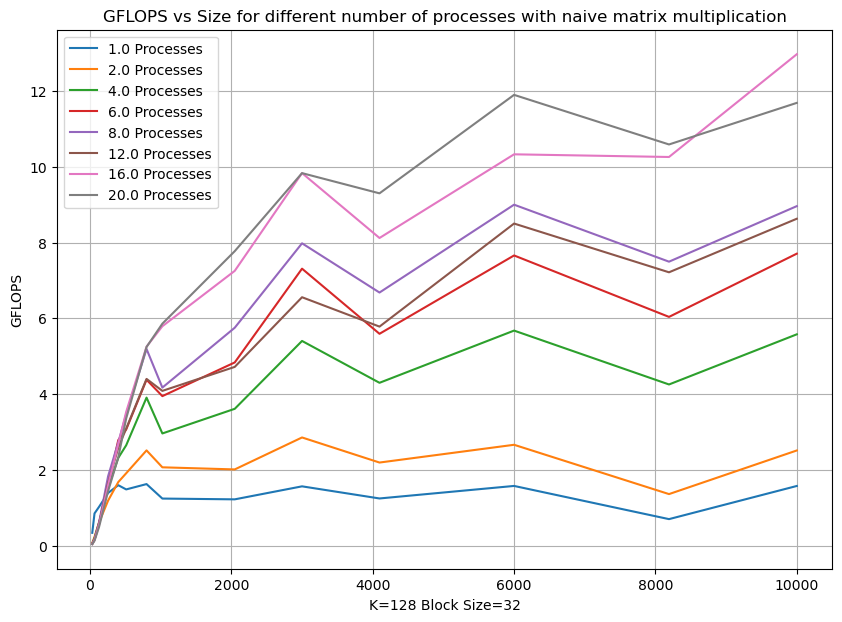
\includegraphics[width=0.4\textwidth]{resources/rettangolari_k128_naive.png}
    \caption{Prestazioni ottenute con matrici rettangolari K=128 e prodotto naive.}
    \label{fig:rect_k128_matrix_naive}
\end{figure}
\begin{figure}[H]
    \centering
    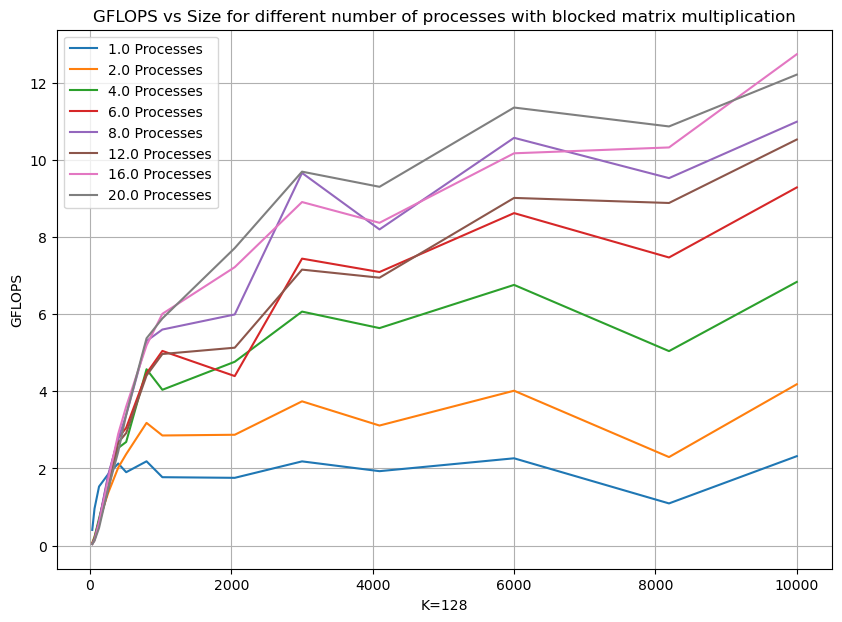
\includegraphics[width=0.4\textwidth]{resources/rettangolari_k128_blocked.png}
    \caption{Prestazioni ottenute con matrici rettangolari K=128 e prodotto column blocked.}
    \label{fig:rect_k128_matrix_blocked}
\end{figure}
\begin{figure}[H]
    \centering
    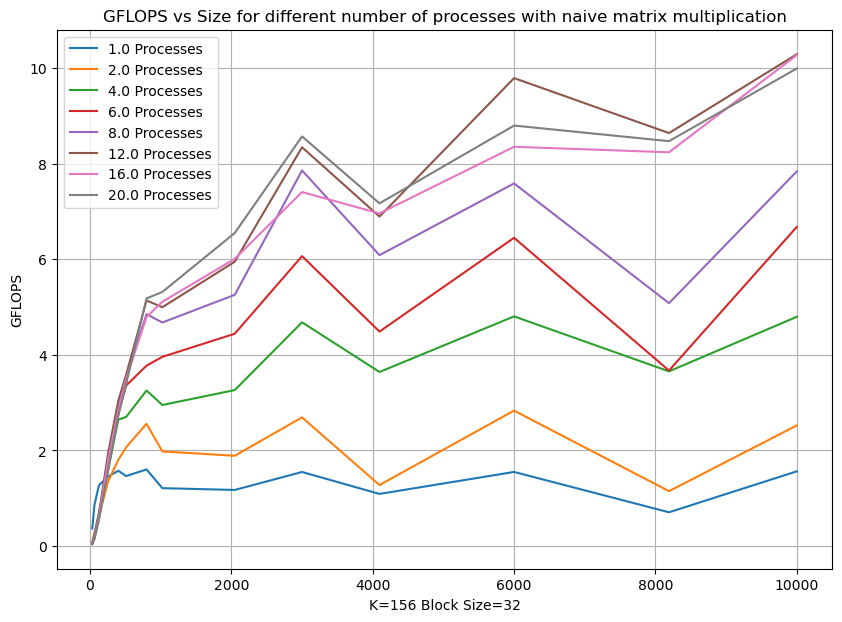
\includegraphics[width=0.4\textwidth]{resources/rettangolari_k156_naive.png}
    \caption{Prestazioni ottenute con matrici rettangolari K=156 e prodotto naive.}
    \label{fig:rect_k156_matrix_naive}
\end{figure}
\begin{figure}[H]
    \centering
    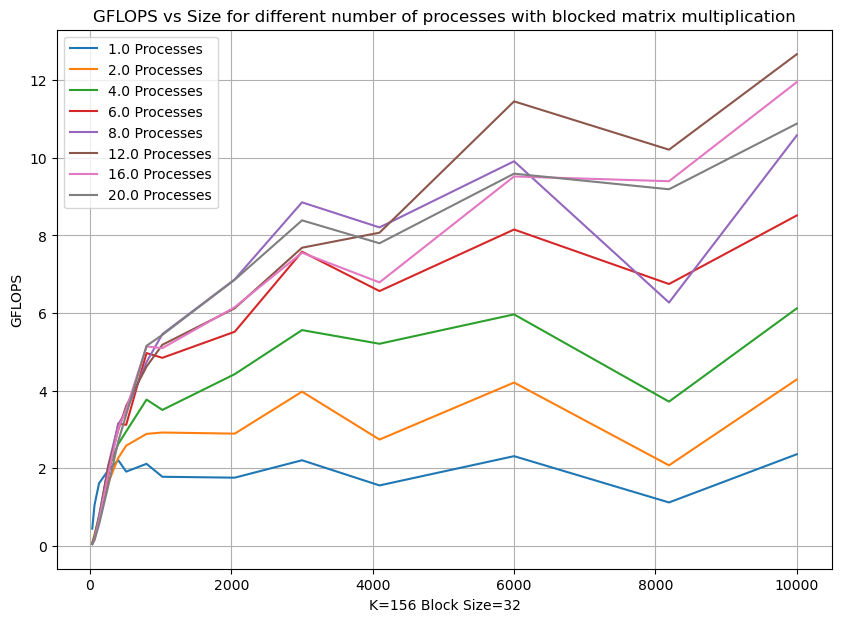
\includegraphics[width=0.4\textwidth]{resources/rettangolari_k156_blocked.png}
    \caption{Prestazioni ottenute con matrici rettangolari K=156 e prodotto column blocked.}
    \label{fig:rect_k156_matrix_blocked}
\end{figure}

\begin{figure}[H]
    \centering
    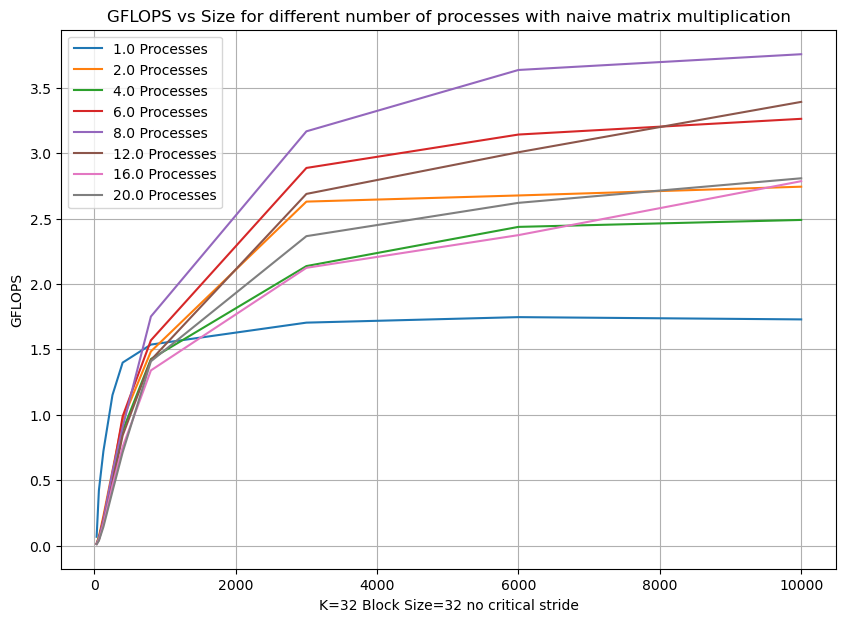
\includegraphics[width=0.4\textwidth]{resources/rect_k32_naive_nocrit.png}
    \caption{Prestazioni ottenute con matrici rettangolari K=32 e prodotto naive. senza critical stride}
    \label{fig:rect_k32_matrix_naive_nocrit}
\end{figure}
\begin{figure}[H]
    \centering
    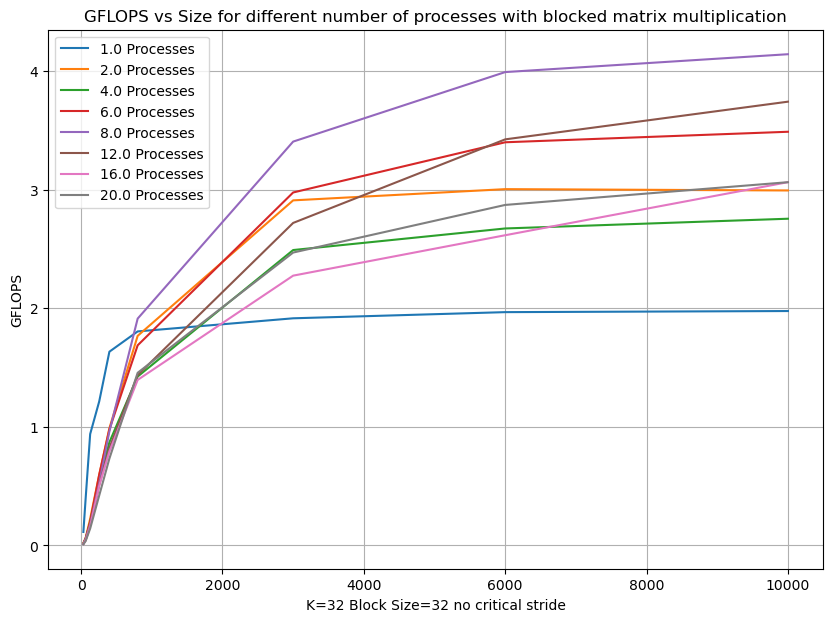
\includegraphics[width=0.4\textwidth]{resources/rect_k32_blocked_nocrit.png}
    \caption{Prestazioni ottenute con matrici rettangolari K=32 e prodotto column blocked senza critical stride.}
    \label{fig:rect_k32_matrix_blocked_nocrit}
\end{figure}
\begin{figure}[H]
    \centering
    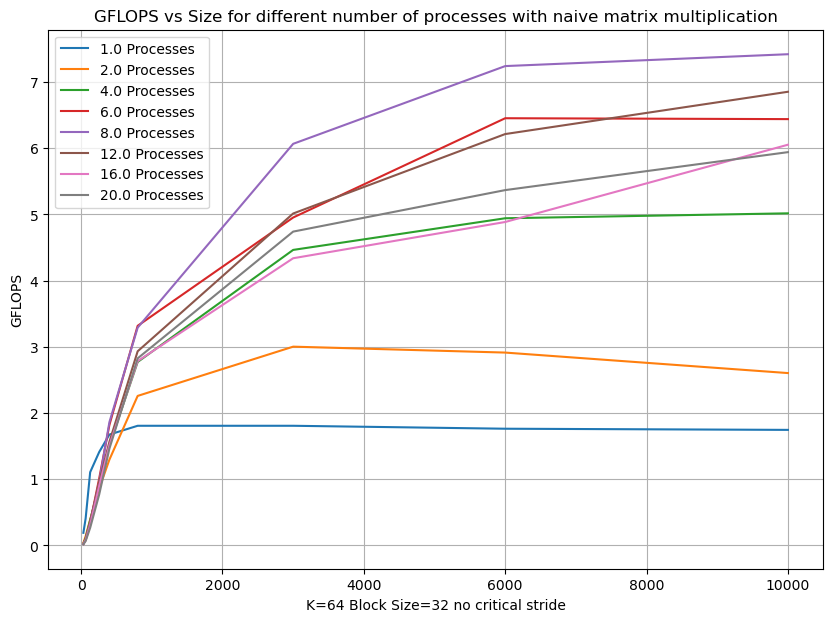
\includegraphics[width=0.4\textwidth]{resources/rect_k64_naive_nocrit.png}
    \caption{Prestazioni ottenute con matrici rettangolari K=64 e prodotto naive senza critical stride.}
    \label{fig:rect_k64_matrix_naive_nocrit}
\end{figure}
\begin{figure}[H]
    \centering
    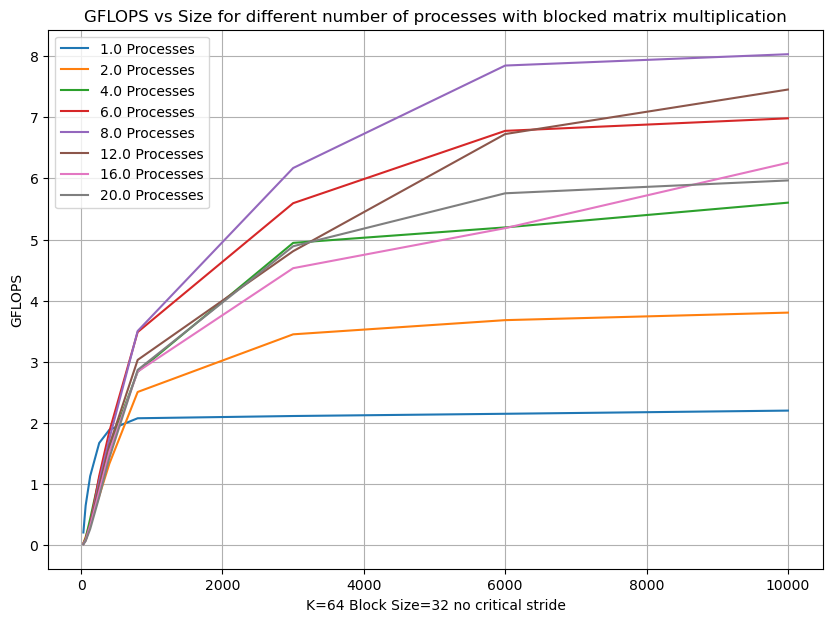
\includegraphics[width=0.4\textwidth]{resources/rect_k64_blocked_nocrit.png}
    \caption{Prestazioni ottenute con matrici rettangolari K=64 e prodotto column blocked senza critical stride.}
    \label{fig:rect_k64_matrix_blocked_nocrit}
\end{figure}
\begin{figure}[H]
    \centering
    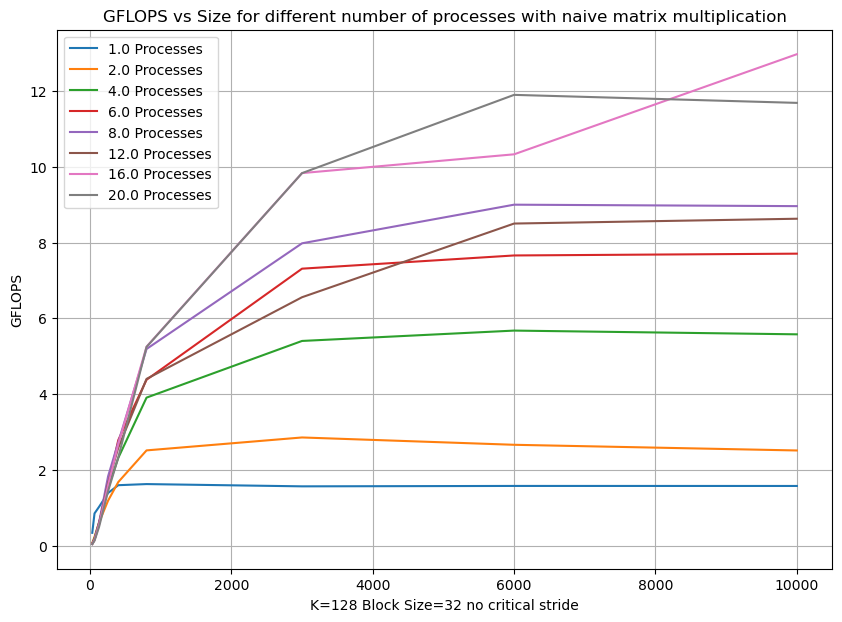
\includegraphics[width=0.4\textwidth]{resources/rect_k128_naive_nocrit.png}
    \caption{Prestazioni ottenute con matrici rettangolari K=128 e prodotto naive senza critical stride.}
    \label{fig:rect_k128_matrix_naive_nocrit}
\end{figure}
\begin{figure}[H]
    \centering
    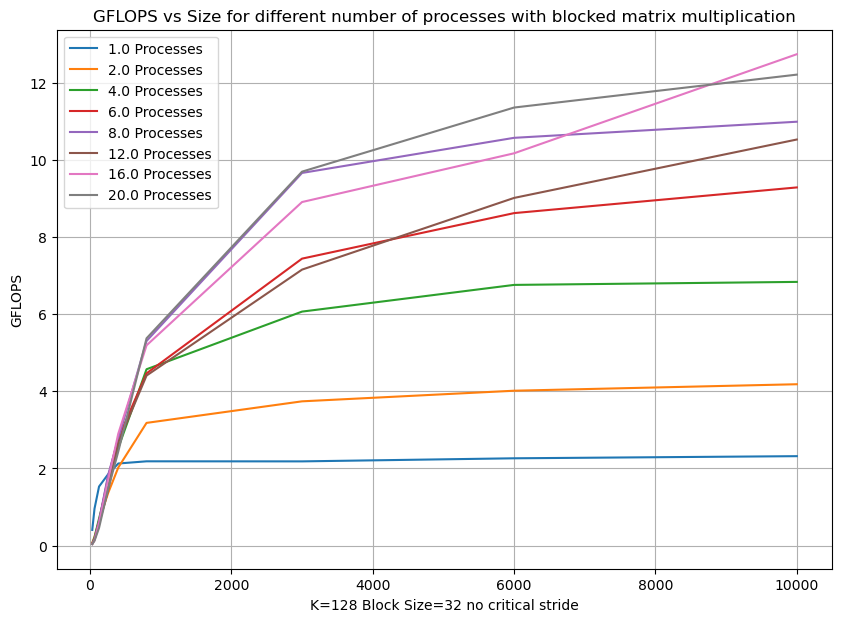
\includegraphics[width=0.4\textwidth]{resources/rect_k128_blocked_nocrit.png}
    \caption{Prestazioni ottenute con matrici rettangolari K=128 e prodotto column blocked senza critical stride.}
    \label{fig:rect_k128_matrix_blocked_nocrit}
\end{figure}
\begin{figure}[H]
    \centering
    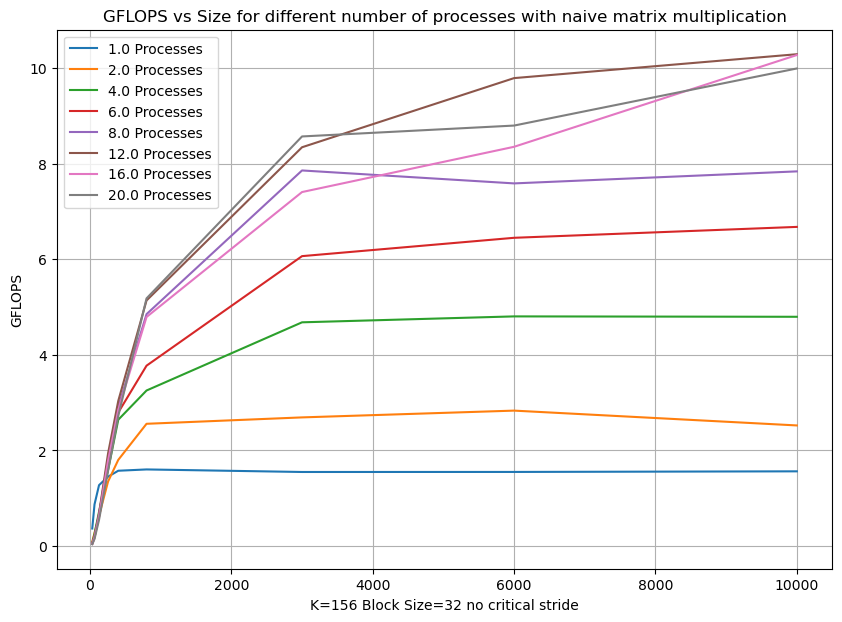
\includegraphics[width=0.4\textwidth]{resources/rect_k156_naive_nocrit.png}
    \caption{Prestazioni ottenute con matrici rettangolari K=156 e prodotto naive senza critical stride.}
    \label{fig:rect_k156_matrix_naive_nocrit}
\end{figure}
\begin{figure}[H]
    \centering
    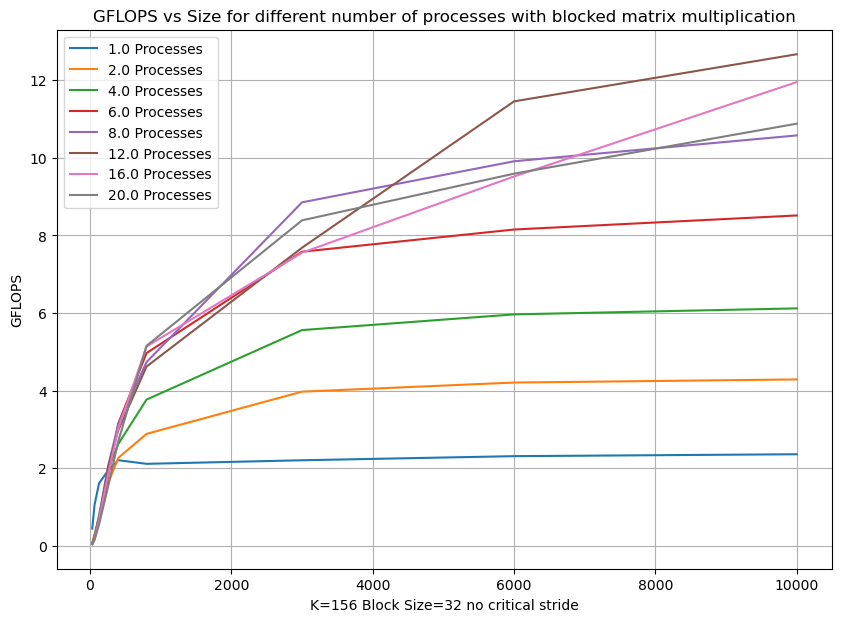
\includegraphics[width=0.4\textwidth]{resources/rect_k156_blocked_nocrit.png}
    \caption{Prestazioni ottenute con matrici rettangolari K=156 e prodotto column blocked senza critical stride.}
    \label{fig:rect_k156_matrix_blocked_nocrit}
\end{figure}
%RISULTATI CUDA
\subsection{CUDA}
Analizziamo ora le prestazioni ottenute dalle diverse versioni del codice CUDA.\\
\subsubsection{Matrici quadrate}
Mettendo a confronto le prestazioni delle 3 versioni del codice tra loro (Fig. \ref{fig:square_matrix}) si può notare immediatamente che la versione 3 è quella che ha prestazioni migliori, questo è dovuto al fatto che essa sfrutta al meglio la shared memory e riduce il numero di accessi alla memoria globale, come spiegato in precedenza. 
Invece la versione 2 ha delle performance peggiori rispetto alla versione 1, nonostante ci si aspettasse un miglioramento. 
Questo strano comportamento potrebbe essere dovuto al fatto che la versione 2 ha un overhead maggiore di memoria rispetto alla versione 1 in quanto deve mantenere una matrice ausiliaria dei risultati parziali più grande e questo potrebbe avere un impatto maggiore rispetto al numero di sincronizzazioni in più della versione 1. Inoltre un'altra motivazione potrebbe essere che dato che nella versione 2 del codice c'è una complessità aggiuntiva dovuta alla necessità di gestire un numero di colonne diverso da 1, l'aggiunta di codice per gestire questa complessità potrebbe aver portato a ridurre i benefici introdotti e quindi ad ottenere delle prestazioni minori.\\
\begin{figure}[H]
    \centering
    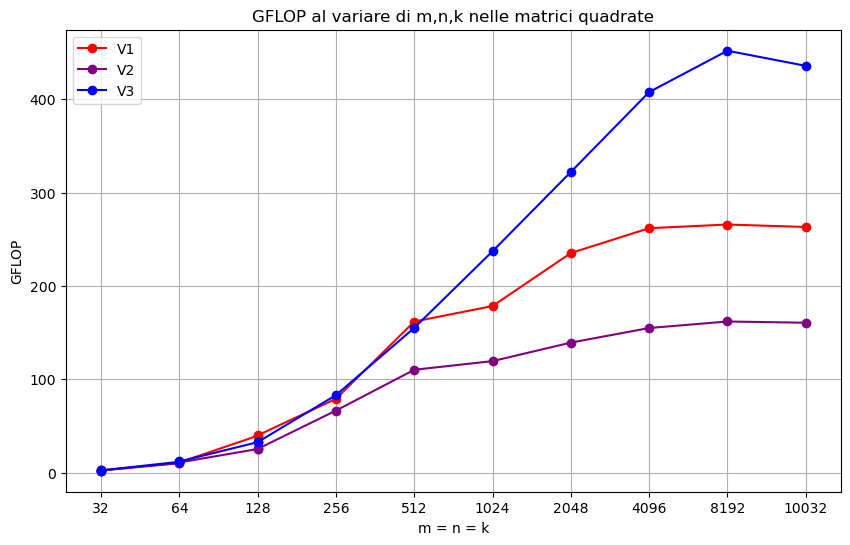
\includegraphics[width=0.5\textwidth]{resources/gpu_matrix_square.png}
    \caption{Prestazioni ottenute con matrici quadrate.}
    \label{fig:square_matrix}
\end{figure}
\subsubsection{Matrici rettangolari}
Per quanto riguarda le matrici rettangolari, si può notare un calo considerevole delle prestazioni. Questo comportamento è probabilmente dovuto al fatto che nelle implementazioni ogni blocco lavora su una singola riga della colonna A alla volta, dividendola per il numero di thread in quel blocco. Dato che ogni riga della matrice A è grande k, e negli esperimenti k varia da 32 a 156, questi sono tutti valori più piccoli della dimensione dei blocchi che è settata a 256. Quindi ci saranno molti thread per ogni blocco che non fanno nulla, portandosi però dietro l'overhead di averli creati. Infatti come si può notare le prestazioni peggiorano sempre più al diminuire del valore di k proprio perché il numero di thread inutili aumenta. E questo succede in tutte le versioni del codice proprio perchè utilizzano tutte lo stesso meccanismo di calcolo.\\

\begin{figure}[H]
    \centering
    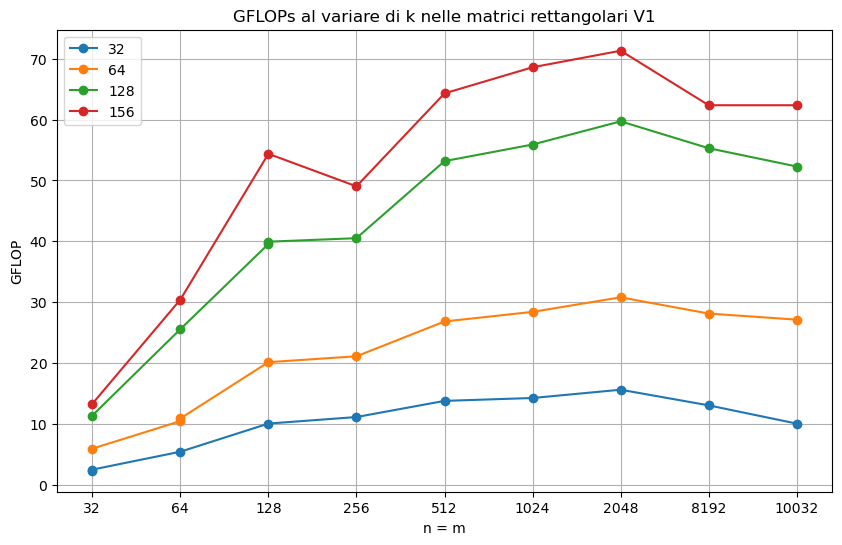
\includegraphics[width=0.5\textwidth]{resources/gpu_matrix_rect_perfv1.png}
    \caption{Prestazioni ottenute con matrici rettangolari nella versione 1.}
    \label{fig:rect_matrix_v1}
\end{figure}
\begin{figure}[H]
    \centering
    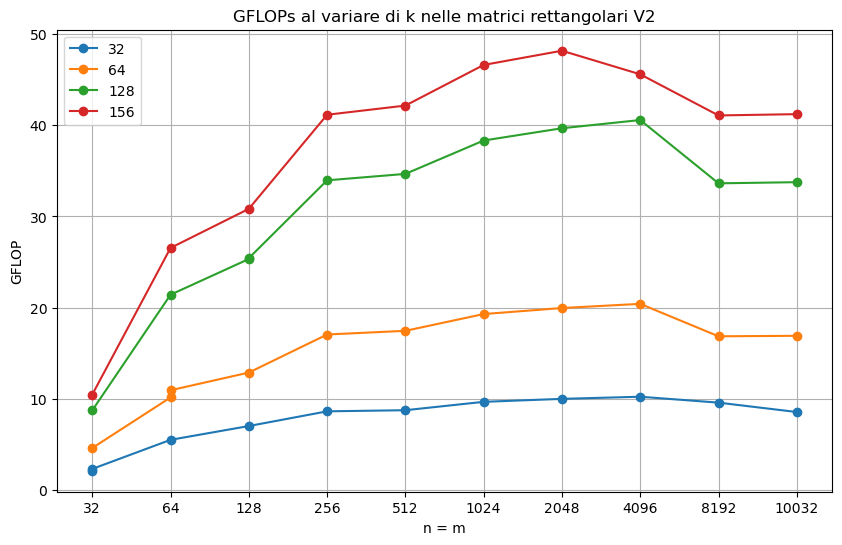
\includegraphics[width=0.5\textwidth]{resources/gpu_matrix_rect_perfv2.png}
    \caption{Prestazioni ottenute con matrici rettangolari nella versione 2.}
    \label{fig:rect_matrix_v2}
\end{figure}
\begin{figure}[H]
    \centering
    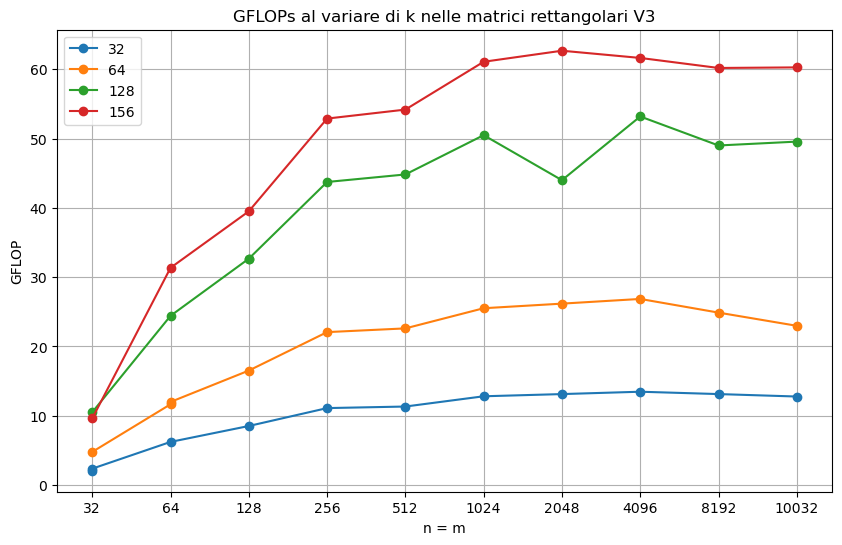
\includegraphics[width=0.5\textwidth]{resources/gpu_matrix_rect_perfv3.png}
    \caption{Prestazioni ottenute con matrici rettangolari nella versione 3.}
    \label{fig:rect_matrix_v3}
\end{figure}
\subsubsection{MPI+CUDA}
Per quanto riguarda le prestazioni ottenute con la soluzione MPI+CUDA bisogna premettere che esse riportano vari limiti intrinsechi:
\begin{itemize}
    \item Nel server dove sono stati fatti gli eseperimenti è presente una sola GPU, e già questo comporta una limitazione notevole dato che il vantaggio di utilizzare la soluzione MPI+CUDA è proprio quello di poter utilizzare le GPU di più server, quindi in questo caso non si sta sfruttando appieno il potenziale della soluzione.
    \item Dato la GPU è una sola quando i processi andranno a tentare di eseguire concorrentemente il nucleo di calcolo su CPU, essi verranno serializzati e quindi non si avrà un vero vantaggio dovuto alla parallelizzazione tra varie GPU
    \item Le prestazioni calcolate, al contrario del caso solo CUDA contengono anche il conteggio del trasferimento della memoria RAM alla memoria globale della GPU, quindi non sono confrontabili direttamente con le prestazioni ottenute con la soluzione solo CUDA.
\end{itemize}
Per questa versione è stata utilizzata solo la versione 3 del codice CUDA, in quanto è quella che ha prestazioni migliori.
\subsubsection{Matrici quadrate}
Come si può vedere dal grafico in Fig. \ref{fig:mpi_cuda_square}, come ci si potrebbe aspettare con un solo processo le prestazioni sono migliori proprio perchè c'è meno overhead dovuto alla comunicazione tra i processi, cosa che negli altri casi sarebbe stato dovuto essere controbilanciato dalla parallelizzazione tra varie GPU cosa che non è stato possibile testare, come citato prima. 
Inoltre si può notare un calo notevole ad un certo punto proprio perché siccome è stata conteggiata anche il trasferimento della matrice in memoria della GPU, all'aumentare della dimensione della matrice il tempo di trasferimento aumenta di conseguenza fino a peggiorare le prestazioni. Tuttavia si può comunque notare un notevole miglioramento rispetto alle prestazioni ottenute con la soluzione solo MPI, ovviamente dovuto all'introduzione della GPU nel calcolo.
\begin{figure}[H]
    \centering
    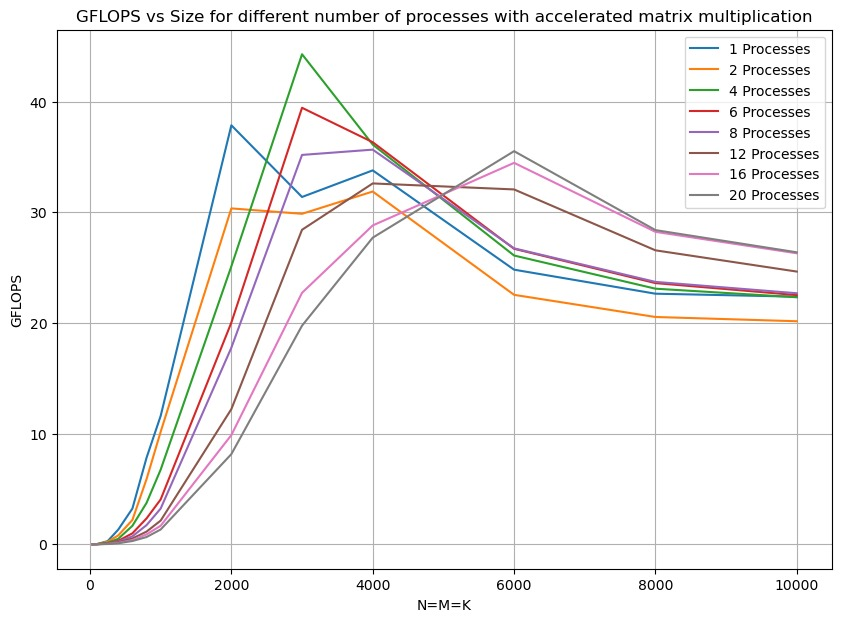
\includegraphics[width=0.5\textwidth]{resources/mpi_cuda_square.jpg}
    \caption{Prestazioni MPI+CUDA con matrici quadrate.}
    \label{fig:mpi_cuda_square}
\end{figure}
\subsubsection{Matrici rettangolari}
Per quanto riguarda le matrici rettangolari (Fig \ref{fig:mpi_cuda_32}, Fig. \ref{fig:mpi_cuda_64}, Fig. \ref{fig:mpi_cuda_128}, Fig. \ref{fig:mpi_cuda_156}), come nel caso già analizzato nella parte CUDA, si può notare un calo notevole delle prestazioni proprio per gli stessi motivi citati in precedenza. Tuttavia si può notare un trend leggermente diverso nel quale al diminuire di k le prestazioni migliorano al contrario di quello che succedeva con il solo codice CUDA. Questo è probabilmente dovuto al fatto che poiché viene conteggiato anche il trasferimento di memoria nel calcolo esso sia un fattore determinante che aiuta matrici più piccole a ottenere prestazioni migliori.
Inoltre come detto anche nel caso delle matrici quadrate, la versione con un solo processo ha delle prestazioni migliori rispetto alle altre proprio perché i kernel non vengono serializzati e ci sono meno \textit{device sinchronize} dovute alla copia dei dati dalla memoria centrale alla memoria della GPU. Oltretuttto, al contrario del caso quadrato non c'è un punto in cui c'è un calo considerevole delle prestazioni dovuto al trasferimento di memoria, questo è probabilmente dovuto al fatto che le matrici rettangolari sono più piccole e quindi il tempo di trasferimento è minore e non si arriva al punto di annullare la controparte di calcolo.
\begin{figure}[H]
    \centering
    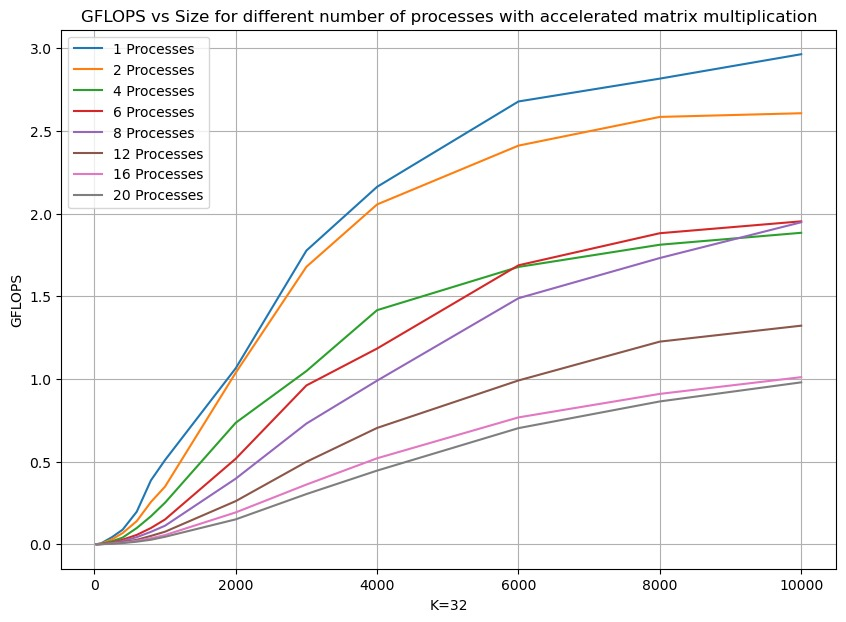
\includegraphics[width=0.45\textwidth]{resources/mpi_cuda_32.jpg}
    \caption{Prestazioni MPI+CUDA con matrici rettangolari K=32.}
    \label{fig:mpi_cuda_32}
\end{figure}
\begin{figure}[H]
    \centering
    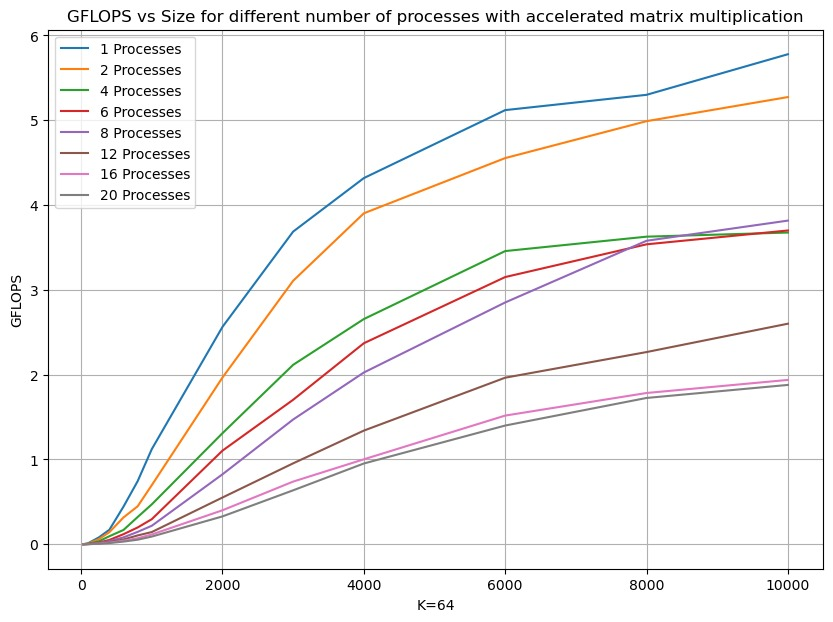
\includegraphics[width=0.45\textwidth]{resources/mpi_cuda_64.jpg}
    \caption{Prestazioni MPI+CUDA con matrici rettangolari K=64.}
    \label{fig:mpi_cuda_64}
\end{figure}
\begin{figure}[H]
    \centering
    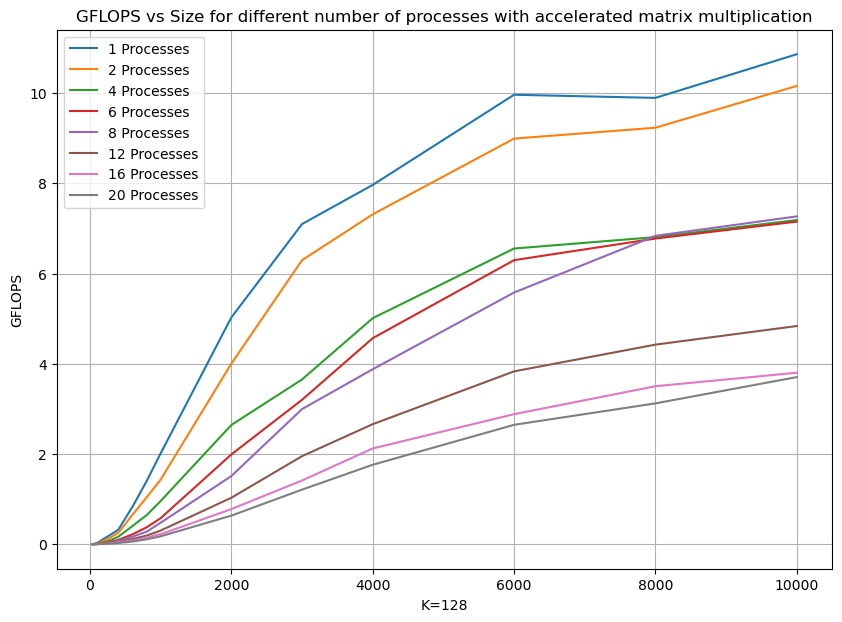
\includegraphics[width=0.45\textwidth]{resources/mpi_cuda_128.jpg}
    \caption{Prestazioni MPI+CUDA con matrici rettangolari K=128.}
    \label{fig:mpi_cuda_128}
\end{figure}
\begin{figure}[H]
    \centering
    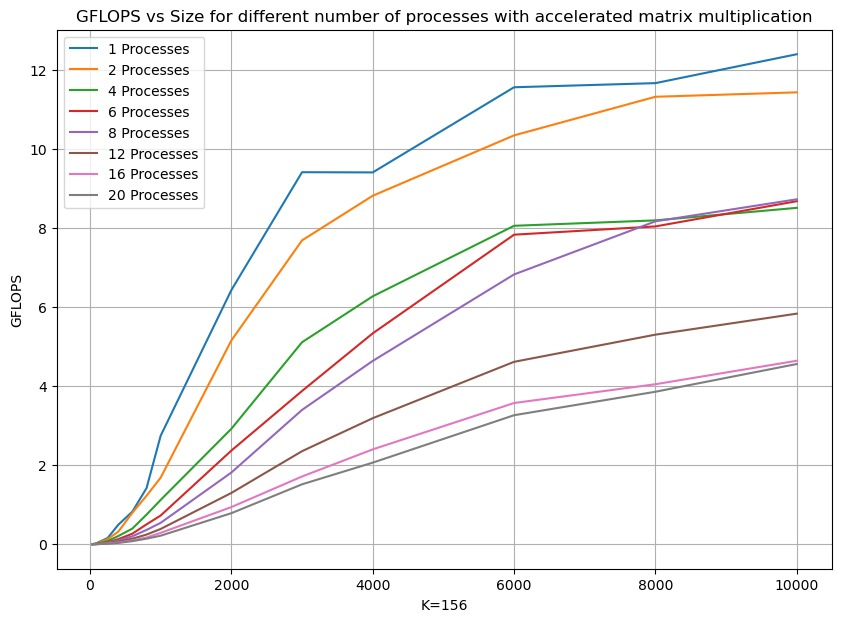
\includegraphics[width=0.45\textwidth]{resources/mpi_cuda_156.jpg}
    \caption{Prestazioni MPI+CUDA con matrici rettangolari K=156.}
    \label{fig:mpi_cuda_156}
\end{figure}
\section{Suddivisione del lavoro}
\begin{itemize}
    \item Luca Falasca: Implementazione del codice CUDA supporto al design della soluzione MPI e all'implementazione del codice MPI+CUDA
    \item Matteo Conti: Implementazione del codice MPI, supporto al design della soluzione CUD e all'implementazione del codice MPI+CUDA
\end{itemize}
\section{Riferimenti}
Codice sorgente
\begin{itemize}
    \item \href{https://github.com/LucaFalasca/ParallelMatrixMultiplication}{https://github.com/LucaFalasca/ParallelMatrixMultiplication}
\end{itemize}
\begin{thebibliography}{00}
    \bibitem{b1} Agner \href{https://www.agner.org/optimize/optimizing_cpp.pdf}{"Optimizing software in C++: An optimization guide for Windows, Linux and Mac platforms"} pp. 91-92.
\end{thebibliography}
\vspace{12pt}

\end{document}